The results from the project are presented in this section. Note that all images of dash-cam footage presented below are not from the SHRP2 data since these cannot be shared and published. Instead, sample free to use videos were used to better show the findings in this section. However, the plots that are presented below were drawn using time-series data acquired from the SHRP2 data. 
% The time-series data used in this report 


\subsection{Image Rectification}
Both intrinsic and extrinsic image rectification were implemented. The results from the image rectification are shown below. 


\subsubsection{Rectification Using Intrinsic Parameters}

Initially, the video was rectified frame by frame using the intrinsic camera parameters. It is important to note that these parameters are camera specific and were acquired for the type of camera used to collect the SHRP2 data.

Figure \ref{fig:image_rectification} shows the result from this rectification on a sample image. Note that this image was resized to be the same resolution and aspect ratio as the videos in the SHRP2 data, hence the grey bars on the top and bottom. 

\begin{figure}[H]
\centering
\begin{minipage}[b]{0.45\linewidth}
    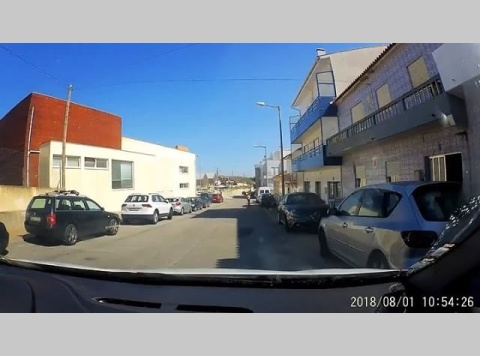
\includegraphics[width=\textwidth]{random_image_extended.jpg}
    \caption*{Distorted image}
\end{minipage}
\begin{minipage}[b]{0.45\linewidth}
    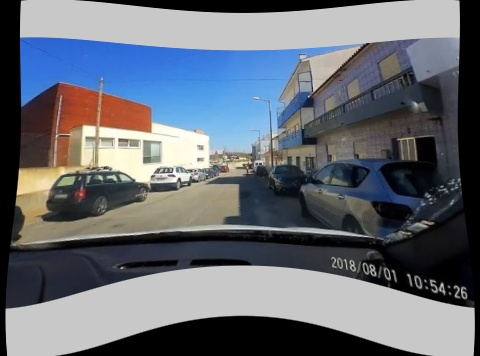
\includegraphics[width = \textwidth]{random_image_rectified.jpg}
    \caption*{Rectified image}
\end{minipage}
\caption{Image rectification using intrinsic parameters}
\label{fig:image_rectification}
\end{figure}

In figure \ref{fig:image_rectification}, it is apparent how the distorted image is stretched and straight objects, like poles, are not straight in the image. The rectification should correct that using the intrinsic parameters. This is not the case in the example presented, where the poles in the rectified image are still not completely straight. This is because the camera used in this example is not the same as the one used to collect the SHARP2 data, and should therefore have different intrinsic parameters.  


\subsubsection{Rectification Using Extrinsic Parameters}

In practice, if the extrinsic calibration is done correctly, then the VP of the lanes should always be moved to the centre of the image. This meant that if the VP is initially not at the centre of the image, the corresponding cam pitch and cam yaw were calculated and used as described in section \ref{sec:meth_ExtrensicParameters} to shift the VP so that it was at the same coordinates as the centre of the image, as shown in Figure \ref{fig:extrParamCali}. Note that only the VP is being transformed, hence the black background in the calibrated figure, which is only drawn to show the effects of the extrinsic calibration. 

\begin{figure}[H]
    \centering
    \begin{minipage}[b]{0.49\linewidth}
    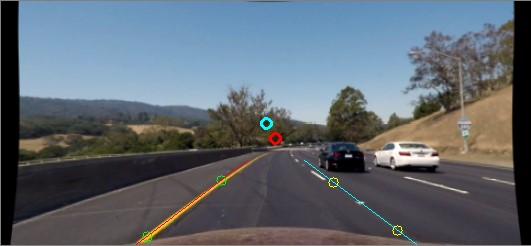
\includegraphics[width=\textwidth]{Figures/vp_initial.jpg}
    \caption*{points before calibration}
    \end{minipage}
    \begin{minipage}[b]{0.49\linewidth}
    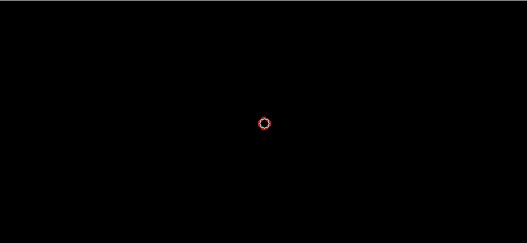
\includegraphics[width=\textwidth]{Figures/vp_fixed.jpg}
    \caption*{points after calibration}
    \end{minipage}
    
    \caption{Image rectification for extrinsic parameters (VP (red) and Image Centre (aqua))}
    \label{fig:extrParamCali}
\end{figure}

\subsection{Lane Tracking}

The three methods of lane tracking previously mentioned were studied. Manual tracking was easy to implement. Fully automatic tracking was more demanding and was not pursued due to the limited time frame of the project. However, semi-automatic was implemented. The results from all three methods are presented below. 
 
\subsubsection{Manual Tracking}

It was found that this method did help in determining the lane placement accurately, given the SV lateral placement in the lane is somewhat constant, as shown in figure \ref{fig:lane_tracking_interpolation} where the user inputs the placement of the lanes in frames 1 and 30, and the program interpolates the placement in the frames between. In this way, the user was able to track the lane in 30 frames, through manually defining the placement in only two frames. 

\begin{figure}[H]
\centering
\captionsetup{justification=centering}
\begin{minipage}[b]{0.45\linewidth}
    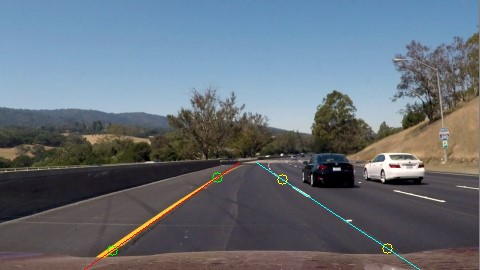
\includegraphics[width=\linewidth]{Figures/interpolation_lane_frame_0.jpg}
    \caption*{User input\\ frame 1}
\end{minipage}
\begin{minipage}[b]{0.45\linewidth}
    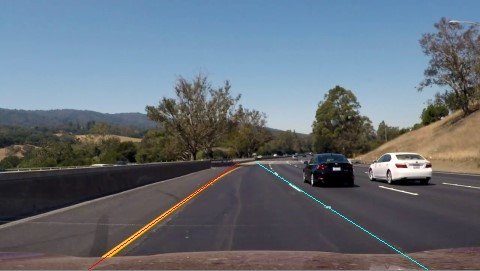
\includegraphics[width=\linewidth]{Figures/interpolation_lane_frame_10.jpg}
    \caption*{Interpolated lane placement\\ frame 10}
\end{minipage}
\vspace{5mm}\\
\begin{minipage}[b]{0.45\linewidth}
    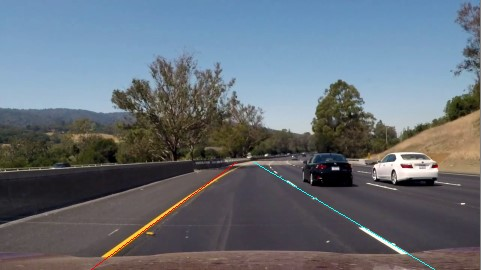
\includegraphics[width=\linewidth]{Figures/interpolation_lane_frame_20.jpg}
    \caption*{Interpolated lane placement\\ frame 20}
\end{minipage}
\begin{minipage}[b]{0.45\linewidth}
    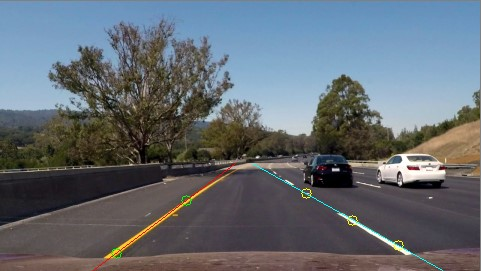
\includegraphics[width=\linewidth]{Figures/interpolation_lane_frame_30.jpg}
    \caption*{User input\\ frame 30}
\end{minipage}
\caption{Results from the interpolation method for lane tracking}
\label{fig:lane_tracking_interpolation}
\end{figure}


\subsubsection{Automatic Tracking}

Four different masking methods were tried, namely gray scale, RGB, HSV and HSL, in order to see which method gives the best results. The lane detection algorithm was tested on three different scenarios, NDS videos containing dashed lanes, see figure \ref{fig:dash_day}, NDS videos containing solid lanes, see figure \ref{fig:solid_day}, and NDS videos recorded during night time, see figure \ref{fig:night}. Three representative videos were used for each of the three scenarios and the results are presented below, in terms of percentage of detected lanes.

\begin{figure}[H]
    \centering    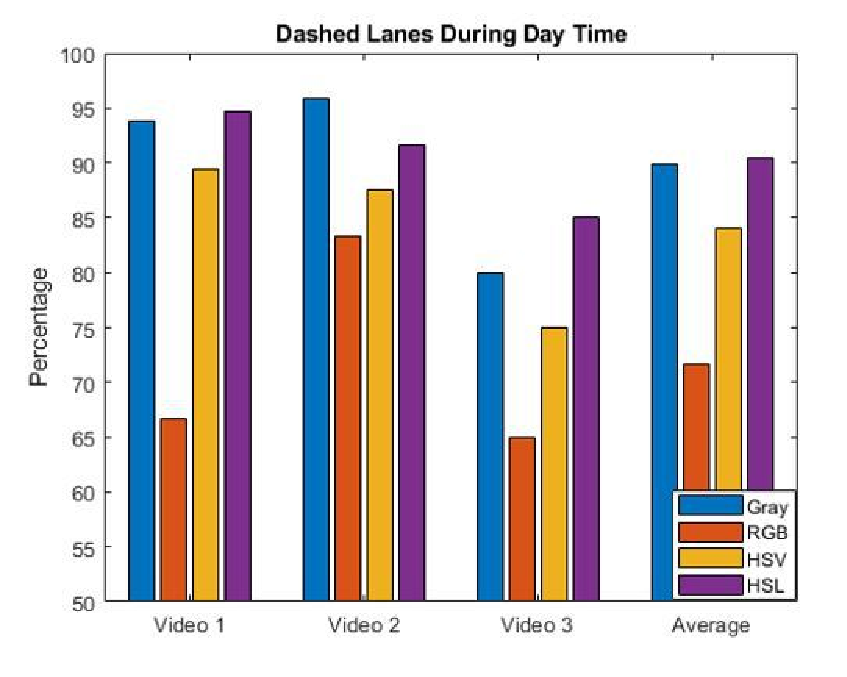
\includegraphics[width = 0.5\textwidth]{Figures/Result_01.pdf}
    \caption{Percentage of detected lanes for different masking methods on dashed lanes during day time}
    \label{fig:dash_day}
\end{figure}

\begin{figure}[H]
    \centering
    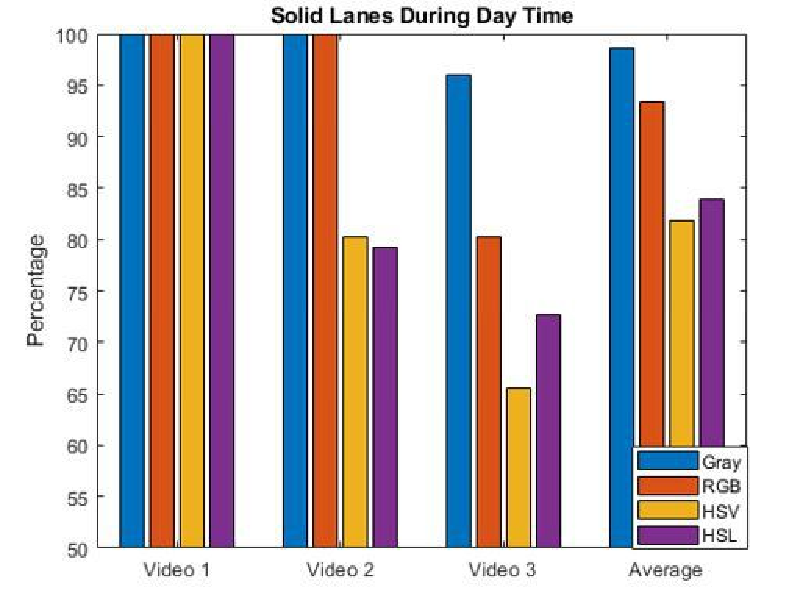
\includegraphics[width = 0.5\textwidth]{Figures/result_02.pdf}
    \caption{Percentage of detected lanes for different masking methods on continuous lanes during day time}
    \label{fig:solid_day}
\end{figure}

\begin{figure}[H]
    \centering
    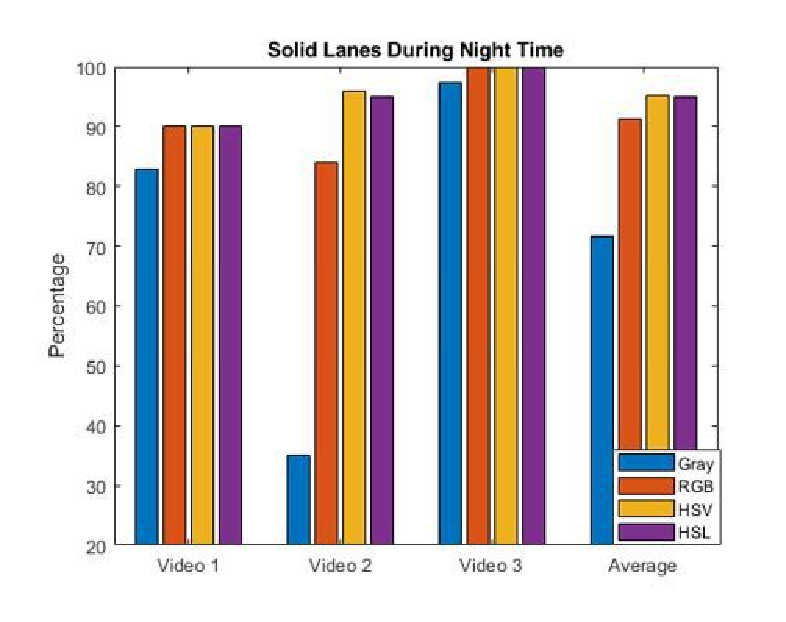
\includegraphics[width = 0.5\textwidth]{Figures/result_03.pdf}
    \caption{Percentage of detected lanes for different masking methods on continuous lanes during night time}
    \label{fig:night}
\end{figure}

Based on this experiment, gray scale seems to be overall best during videos recorded during day time. While HSV masking is more or less equal good as gray scale when it comes to videos recorded during night time.

\paragraph{Misdetection of lanes}
In order to determine how accurate the results presented in the previous section are, the percentage of misdetected lanes for each masking method was calculated. The ROI of the lane detection algorithm was defined in an area of the image where no lanes are present, and the percentage of misdetected lanes for each masking method was assessed. The experiment was done for videos recorded both during day time and videos recorded during night time. The results are presented in Table \ref{tab:misdetection}.


% \begin{figure}[H]
%     \centering
%     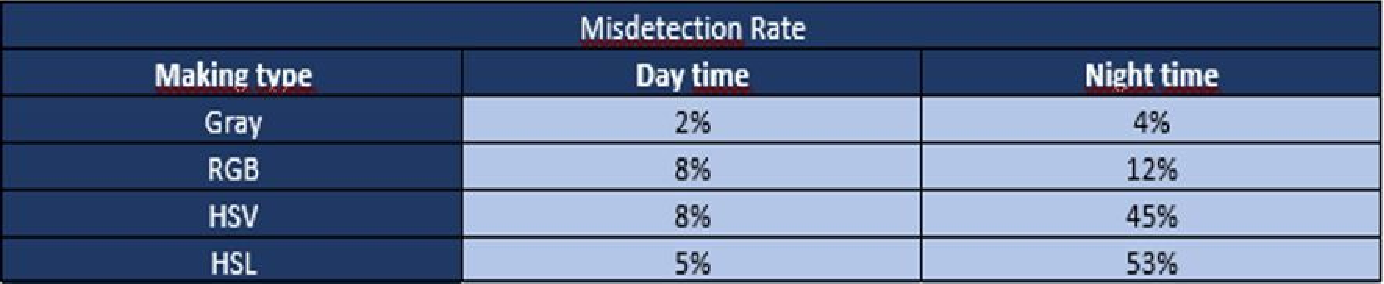
\includegraphics[width = 0.8\textwidth]{Figures/mis-detection.pdf}
%     \caption{Mis-detection of lanes for different masking methods during day and night time expressed in percentages}
%     \label{fig:misdetection}
% \end{figure}

\begin{table}[H]
    \centering
    \begin{tabular}{c|c|c}
         \multicolumn{3}{c}{\textbf{Mis-detectin Rate}} \\ \hline
         Making Type & Day Time $(\%)$ & Night Time $(\%)$ \\ \hline
         Gray & 2 & 4 \\
         RGB & 8 & 12 \\
         HSV & 8 & 45 \\
         HSL & 5 & 53
    \end{tabular}
    \caption{Mis-detection of lanes for different masking methods during day and night time expressed in percentages}
    \label{tab:misdetection}
\end{table}

The result shows that gray scale has by far the smallest percentage of misdetected lanes. The results also show that colour masking causes very high percentage of misdetected lanes during night time. A high misdetection rate leads to misleading result.

\paragraph{Flickering}

The result from the flickering test are present in figure \ref{fig:flick_day} and figure \ref{fig:flick_night}. The result in figure \ref{fig:flick_day} shows that automatic lane detection tends to have less flickering when analyse videos recorded during  day time compared to manual tracking of lanes. However, the result in figure \ref{fig:flick_night} shows that automatic lane detection tends to have more flickering when analyse videos recorded during night time compared to manual tracking of lanes.

\begin{figure}[H]
    \centering
    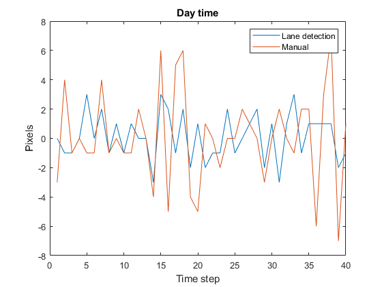
\includegraphics[width = 0.8\textwidth]{Figures/flick2.png}
    \caption{Flickering of the detected lanes during day time for manual tracking and automatic tracking of lanes}
    \label{fig:flick_day}
\end{figure}

\begin{figure}[H]
    \centering
    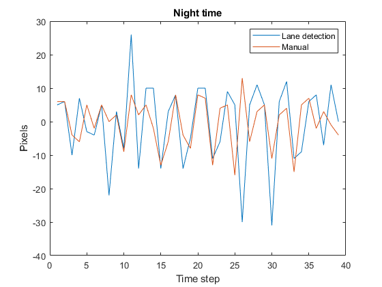
\includegraphics[width = 0.8\textwidth]{Figures/flick1.png}
    \caption{Flickering of the detected lanes during night time for manual tracking and automatic tracking of lanes}
    \label{fig:flick_night}
\end{figure}




\paragraph{Bird's eye transformation}
The figure below shows the perspective transform obtained on a test image. The end co-ordinates of the test image from the original view are selected as source and the destination co-ordinates(the co-ordinates of trapezoidal view as seen in figure of bird's eye transformation) are specified as a separate array. The source and destination on original and bird's view respectively are given as input to a transformation matrix. This is followed by a function named warped perspective in openCV library which modifies the translation,scaling and rotation matrix to give the resulting bird's eye view transformation as shown in the figure below.

\begin{figure}[H]
    \centering
    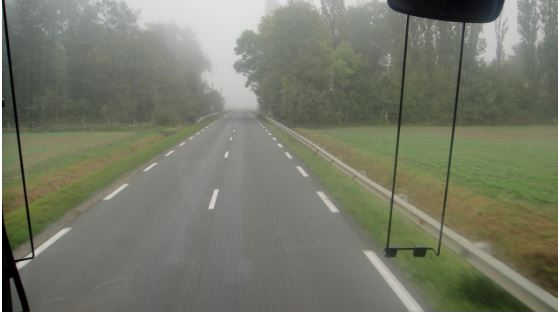
\includegraphics[width = 0.7\textwidth]{Figures/Originalview.JPG}
    \caption{Original view}
    \label{fig:my_label1}
\end{figure}
\begin{figure}[H]
    \centering
    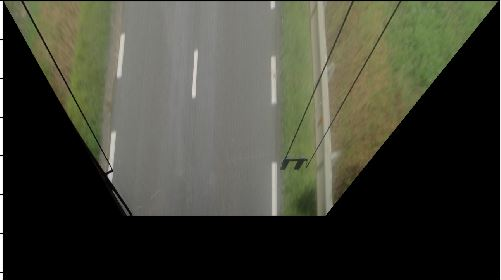
\includegraphics[width = 0.7\textwidth]{Figures/Bird'sview.JPG}
    \caption{Bird's eye transformation}
    \label{fig:my_label2}
\end{figure}
\subsection{Heading Angle}
Only the triangulation method was implemented for the heading angle. Even though this method relied on the user to define the POV wheel placement on the ground, it proved to be the easiest to implement and provided good results, as presented below.

% \subsubsection{Method 1 for Heading Angle: Triangulation}

Figure clearly shows how the POV is maneuvering: first by having a small heading angle which increases to reach a maximum during the maneuver and then decreases back to a low value when the POV is ending the maneuver to continue straight ahead. 

In Figure \ref{fig:heading_angle} and the graphs that follow, "Event 1" refers to the annotation of an event where the SV is changing lanes, while "Event 2" refers to the annotation of an event where the SV stays in its lane (i.e not changing the yaw angle of the camera). It is seen in Figure \ref{fig:heading_angle} that Event 1 seems to have a jumpy behaviour and that is because the SV is changing lanes at the same time as the POV is changing lanes, and because the event takes place on a curved road. Those added to the assumption errors and hence show a more jerky motion of the POV's heading angle.


\begin{figure}[H]
\centering
\begin{minipage}[b]{0.49\textwidth}
    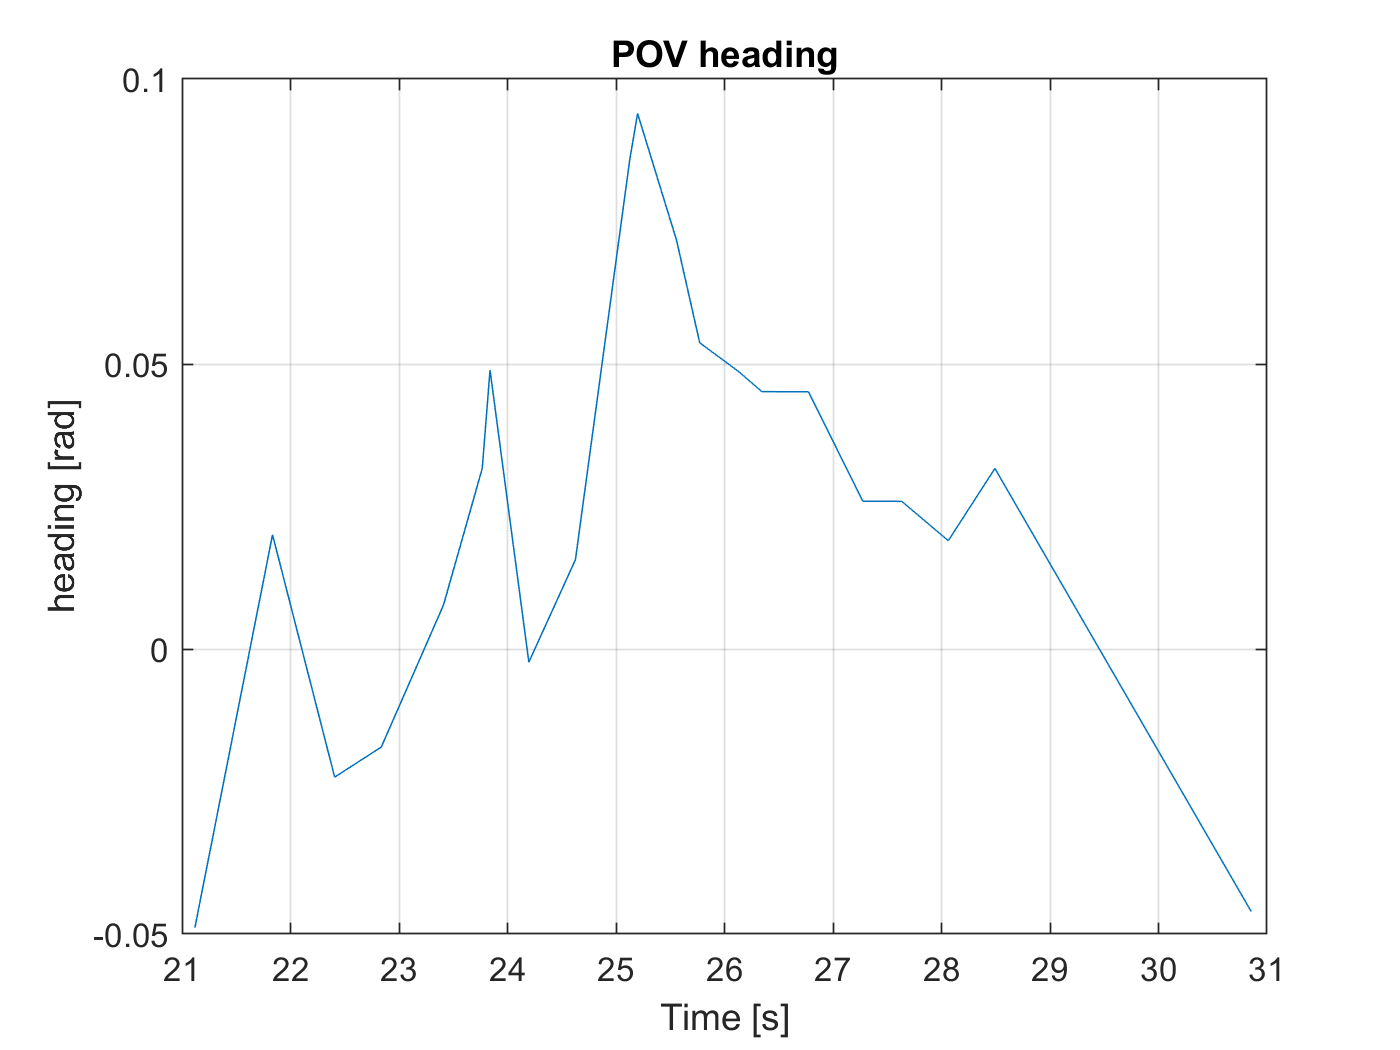
\includegraphics[width=\textwidth]{FiguresMat/pov_heading_10794257.png}
    \caption*{Event 1}
\end{minipage}
\begin{minipage}[b]{0.5\textwidth}
    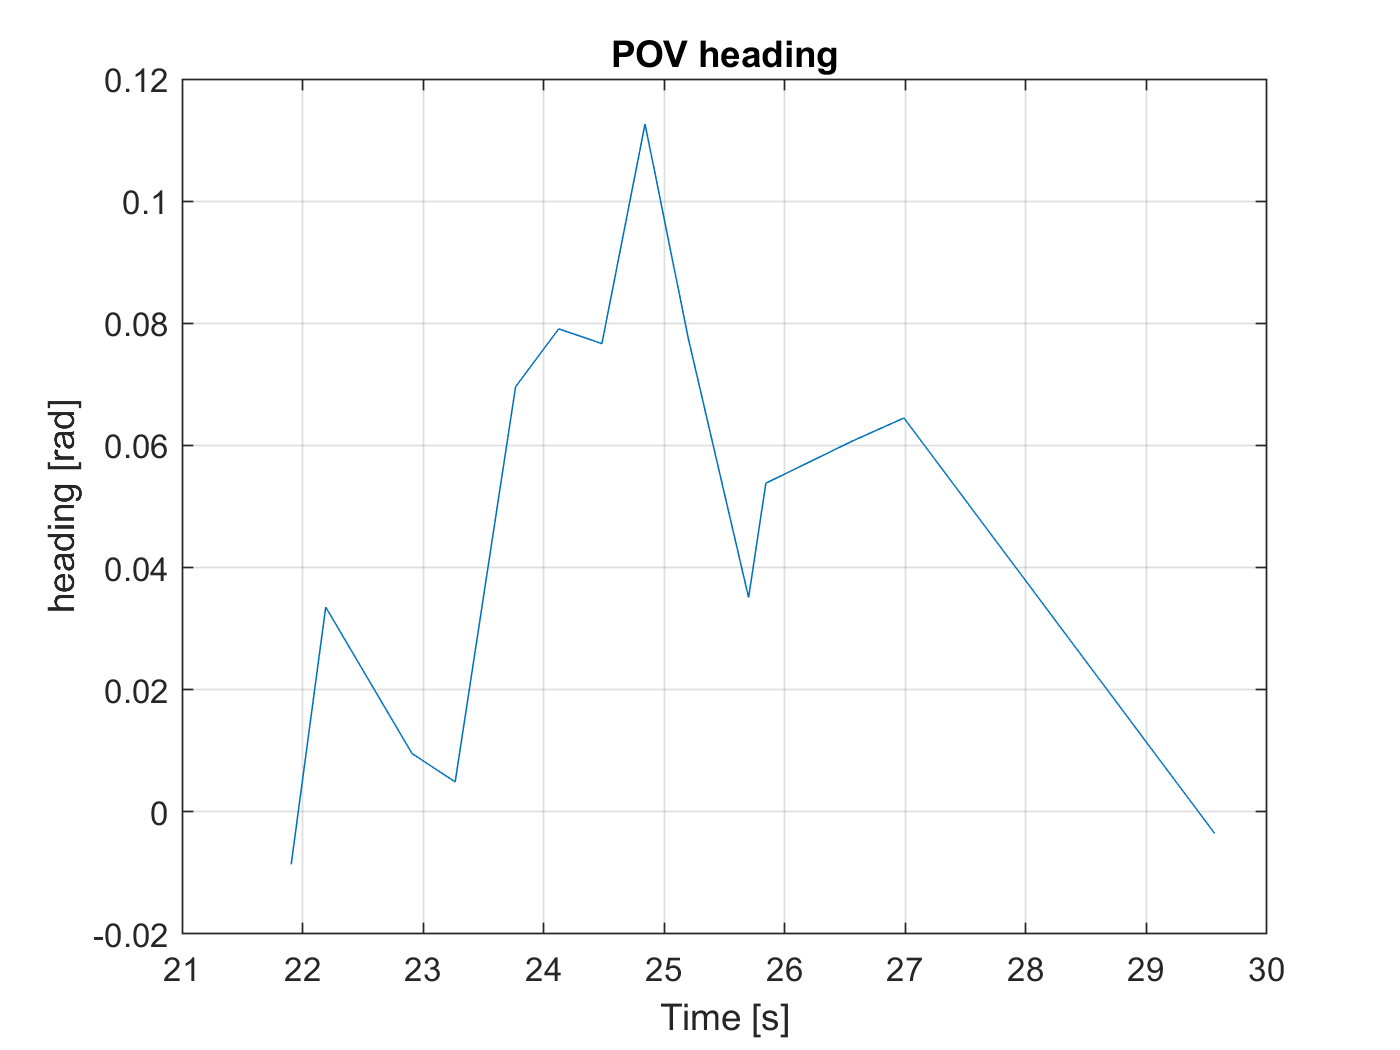
\includegraphics[width=\textwidth]{FiguresMat/pov_heading_116147345.png}
    \caption*{Event 2}
\end{minipage}
\caption{POV Heading Angle}
\label{fig:heading_angle}
\end{figure}

\subsection{Lateral Offset}

The plots presented blow were done for critical lane-changing events in the SHRP2 data that have radar range available. These were the same as "Event 1" and "Event 2" presented earlier.  

\subsubsection{Filtering}

The acquired lateral offset from the annotation tool was used to calculate the lateral offset rate to the POV. It was found that the raw output was not smooth enough and required filtering to gain reasonable lateral offset rate values, as shown in Figures \ref{fig:lat_offset_event1} and \ref{fig:lat_offset_event2}. Better results were acquired after applying two filters to the estimated range before calculating the range rate. Filter specifications are presented below in Table \ref{tab:filters}.

\begin{table}[H]
    \centering
\begin{tabular}{l|l|l}
    \textbf{Name} & \textbf{Type} & \textbf{Specification} \\
    \hline
    filter 1&  Savago & Poly order 2 and window length 11\\
    filter 2& Moving Average & Window length 11 frames
\end{tabular}
    \caption{Filters used on the raw estimated range}
    \label{tab:filters}
\end{table}


\begin{figure}[H]
    \centering
    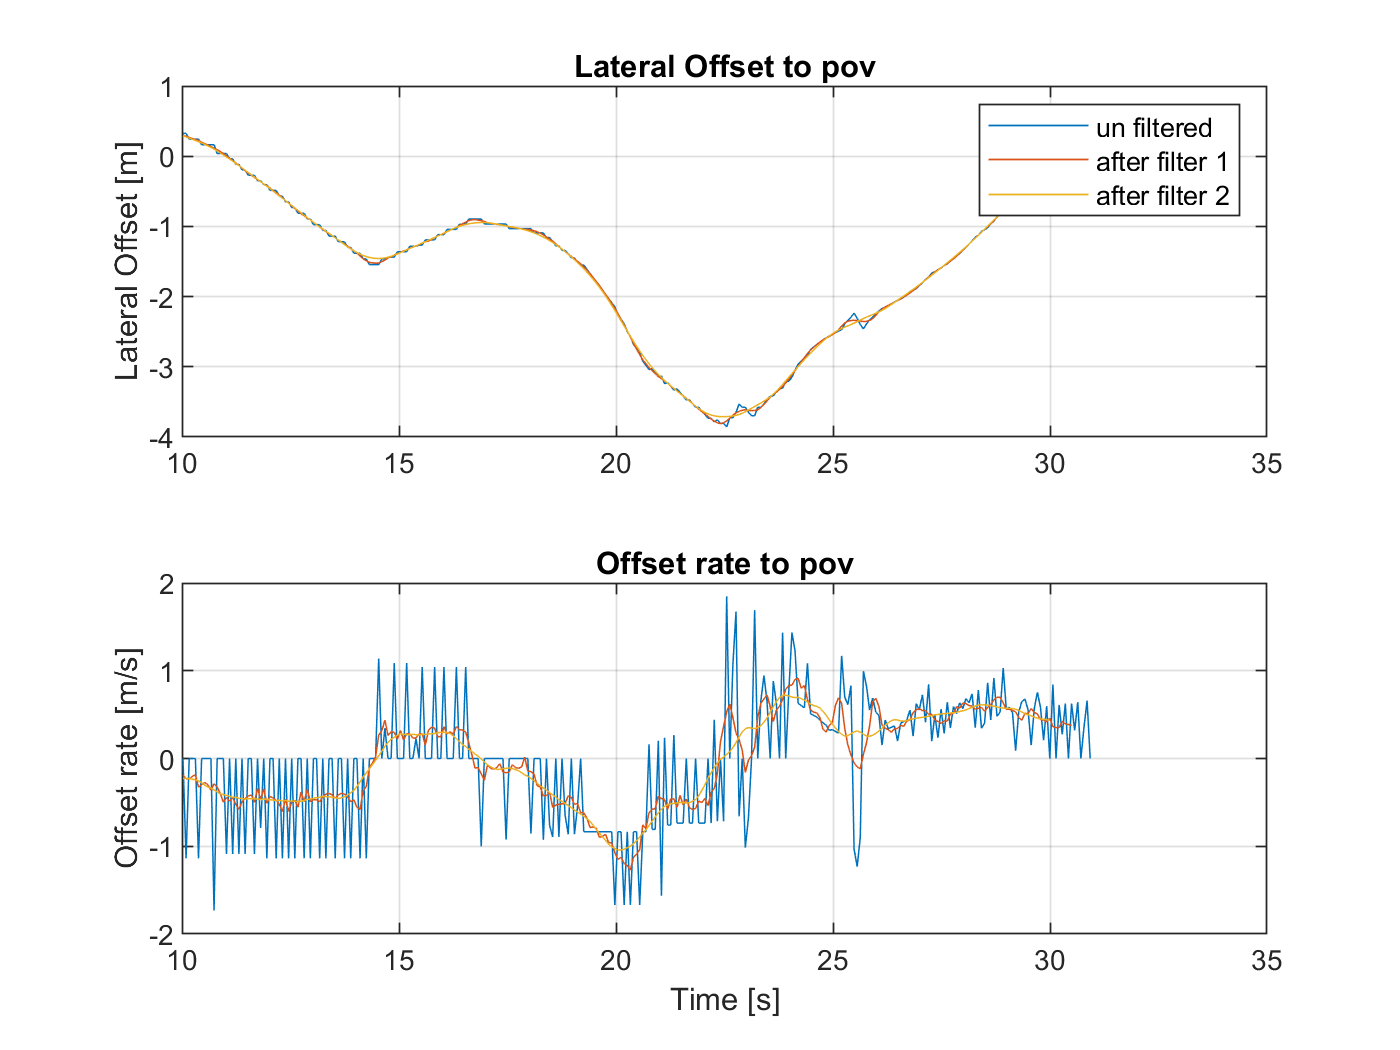
\includegraphics[width=0.8\textwidth]{FiguresMat/filter_compare_lateral_10794257.png}
    \caption{Estimated Lateral offset and offset rate for Event 1}
    \label{fig:lat_offset_event1}
\end{figure}

\begin{figure}[H]
    \centering
    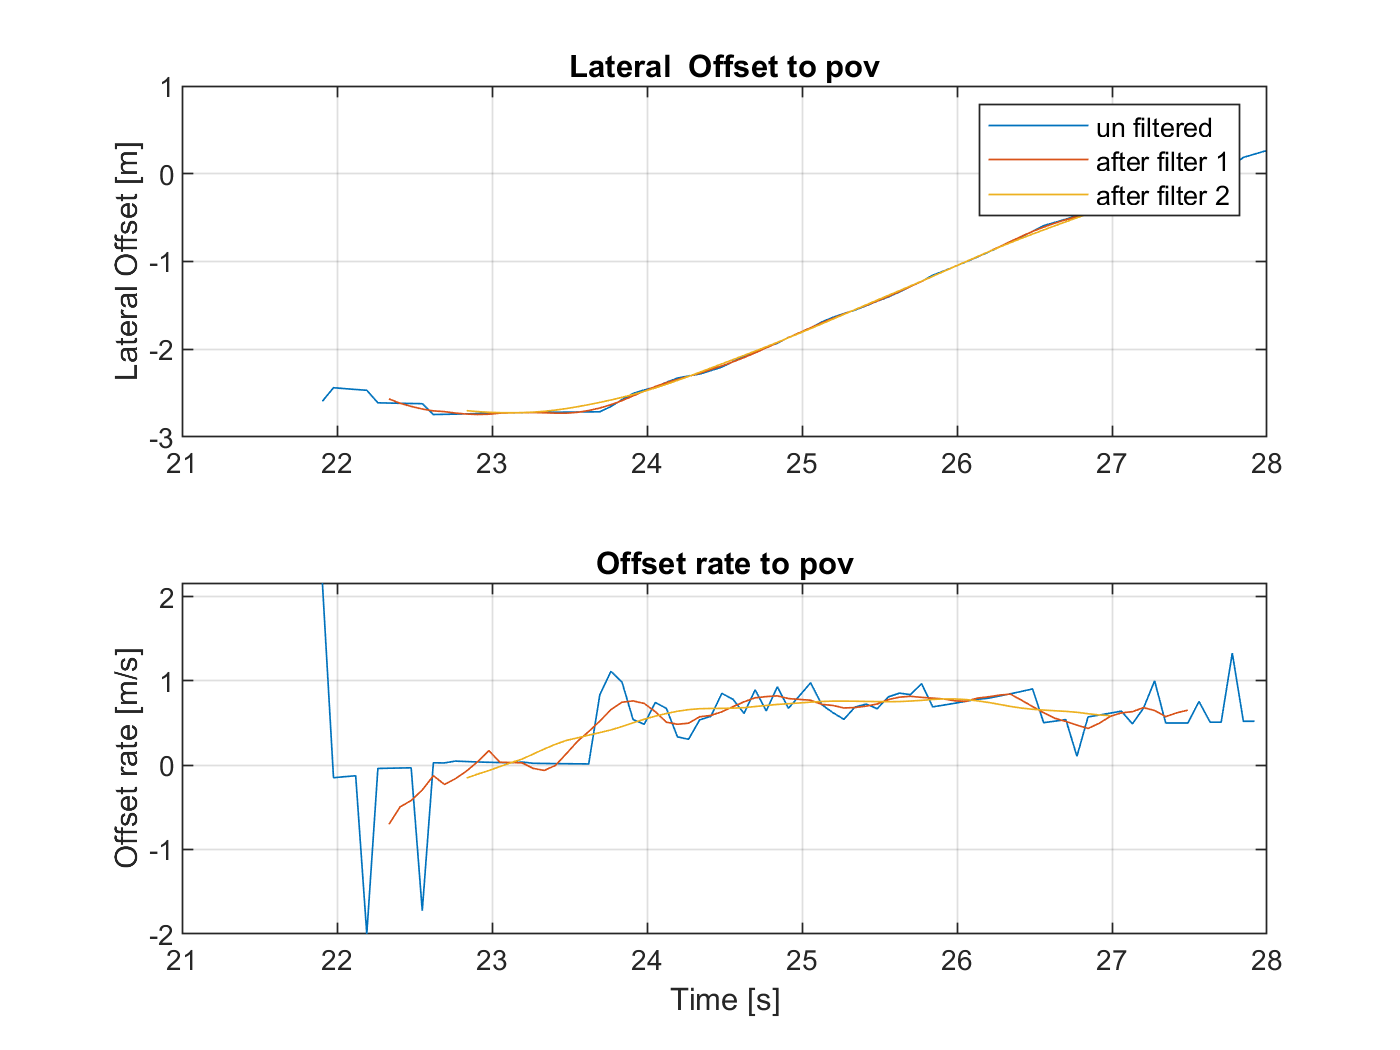
\includegraphics[width=0.8\textwidth]{FiguresMat/filter_compare_lateral_116147345.png}
    \caption{Estimated Lateral offset and offset rate for Event 2}
    \label{fig:lat_offset_event2}
\end{figure}


\subsubsection{Comparing Estimated Lateral Offset to Radar Data}

After filtering, the results of the pixel width method were compared to the available radar data, as shown in Figures \ref{fig:lat_offset_vs_radar_event1} and \ref{fig:lat_offset_vs_radar_event2}. As seen in these figures, the lateral offset gained from the pixel width method followed approximately the same shape as that of the radar data in both events 1 and 2. 

In event 1 of Figure \ref{fig:lat_offset_vs_radar_event1}, it is apparent how the SV was in the same lane as the POV, as the lateral offset was $\approx 0[m]$. The SV changed lane after $\approx 22[s]$, then the POV cut in-front of the SV until the POV was completely in the same lane, as the lateral offset returned to $\approx 0[m]$. 

\begin{figure}[H]
    \centering
    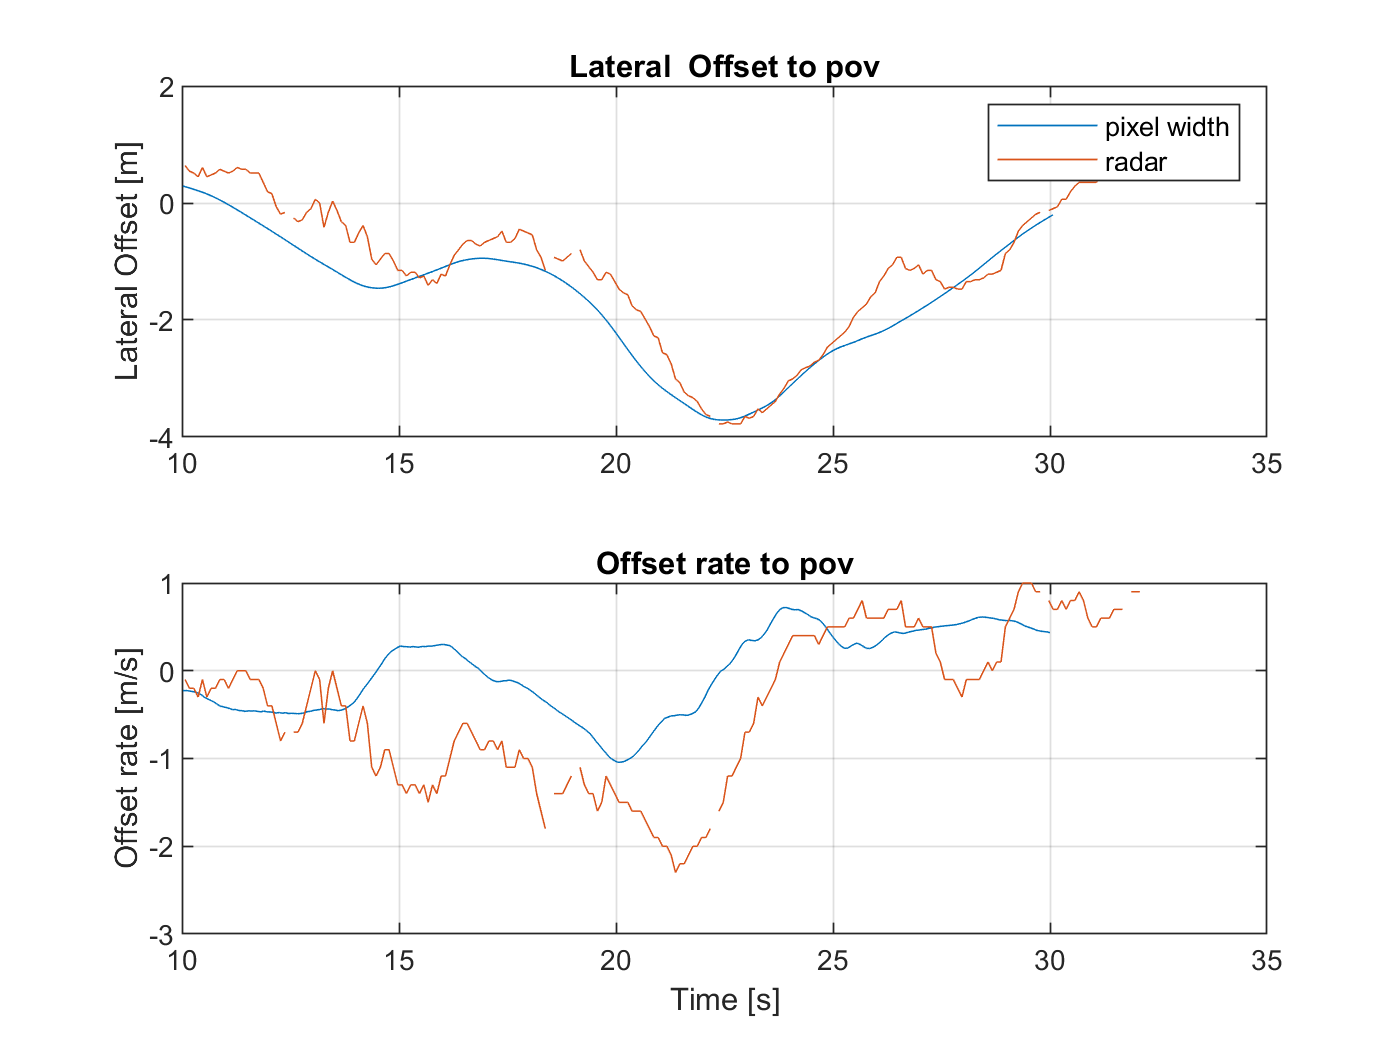
\includegraphics[width=0.8\textwidth]{FiguresMat/radar_compare_lateral_10794257.png}
    \caption{Estimated Lateral Offset vs Radar Data Event 1}
    \label{fig:lat_offset_vs_radar_event1}
\end{figure}

In event 2 of Figure \ref{fig:lat_offset_event2}, it is apparent how the SV was already in a different lane from the POV before the critical event, as the lateral offset was $\approx -3[m]$. After $\approx 24[s]$, the POV started to cut in-front of the SV until the POV is completely in the same lane as the SV, as the lateral offset returned to $\approx 0[m]$

\begin{figure}[H]
    \centering
    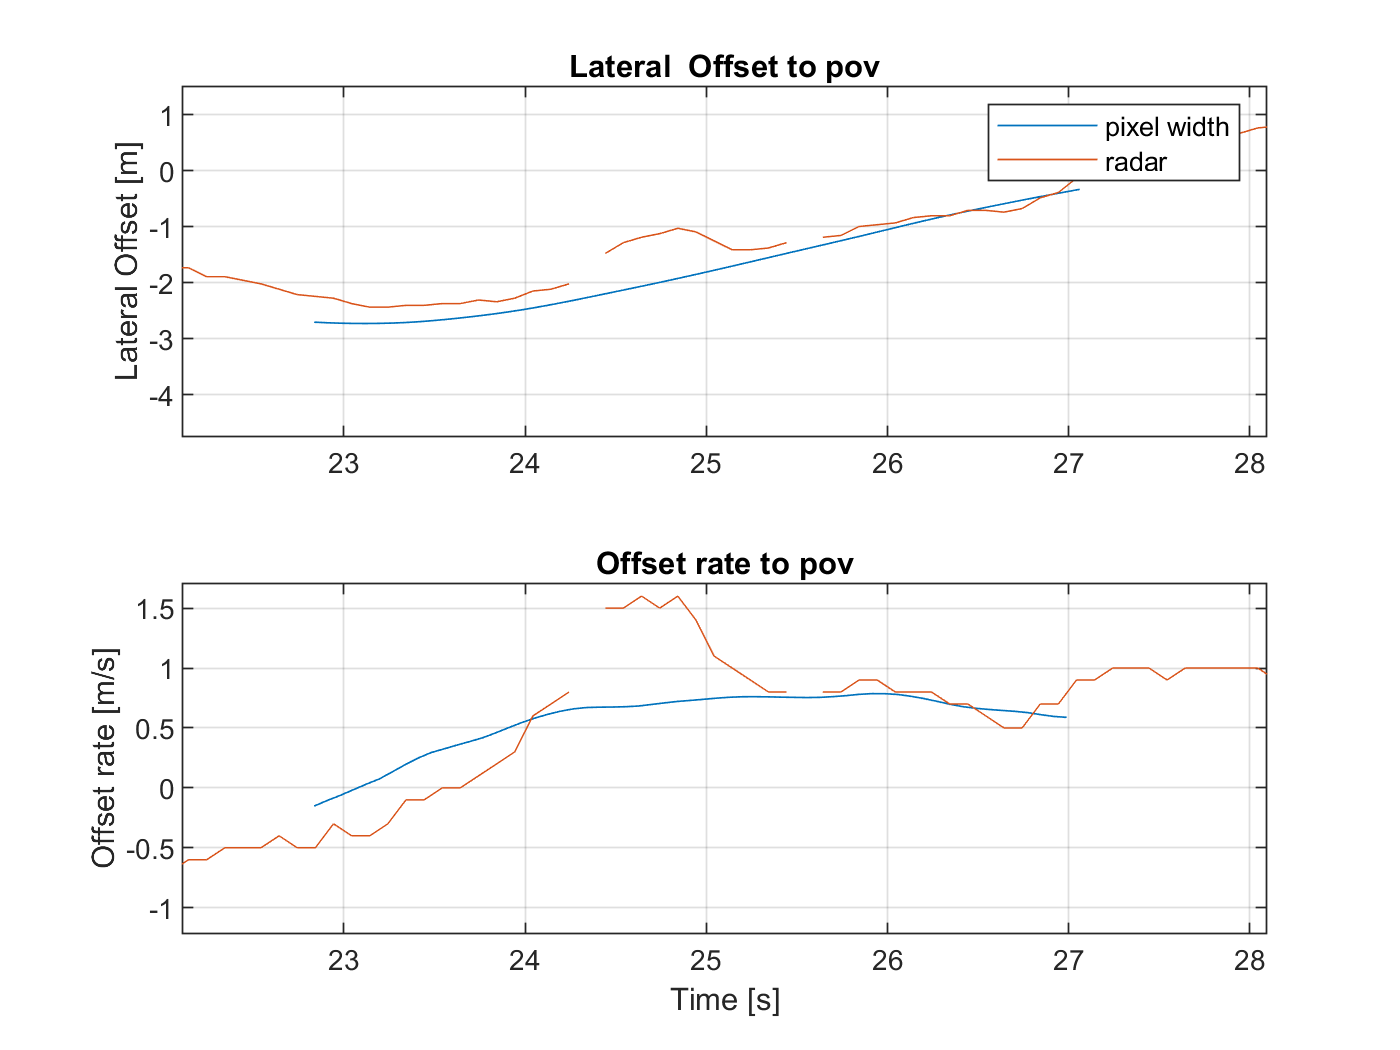
\includegraphics[width=0.8\textwidth]{FiguresMat/radar_compare_lateral_116147345.png}
    \caption{Estimated Lateral Offset vs Radar Data Event 2}
    \label{fig:lat_offset_vs_radar_event2}
\end{figure}

The lateral offset rate, however,  did deviate more from the radar data, but did so more in event 1, where the SV was changing lane before the critical event, compared to event 2, where the SV was in the same lane for the entire duration of the critical event.




% \subsubsection{Method 1 for Lateral Offset}

\subsubsection{Comparing Triangulation method to Pixel Width method and Radar Data}
The results found above were compared to the estimated offset gained from the triangulation method, as presented in Figure \ref{fig:triangulation_comparison_latoffset}. As seen in this figure, the lateral offset using this method in event 1 deviates more from the both radar and the estimated offset gained from the pixel width method. For event 2, however, both methods produce approximately the same results. Due to time constraints, lateral offset rate gained from the triangulation method was not compared to the other results. 

\begin{figure}[H]
    \centering
\begin{minipage}[b]{0.49\textwidth}
    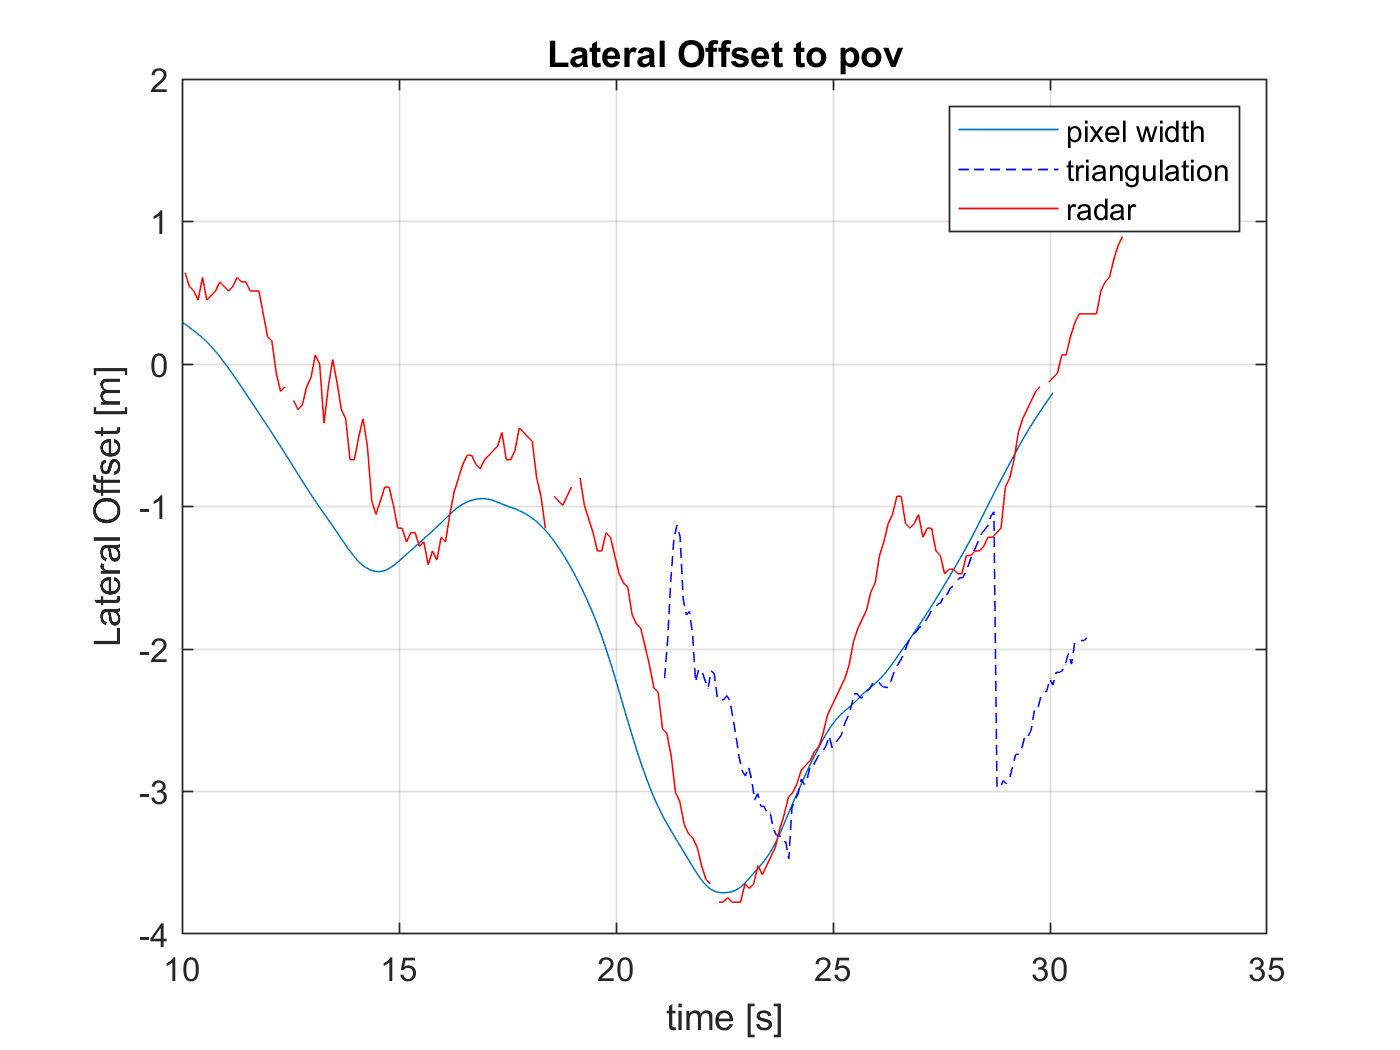
\includegraphics[width=\textwidth]{FiguresMat/homography_comparison_lat_10794257.png}
    \caption*{Event 1}
\end{minipage}
\begin{minipage}[b]{0.50\textwidth}
    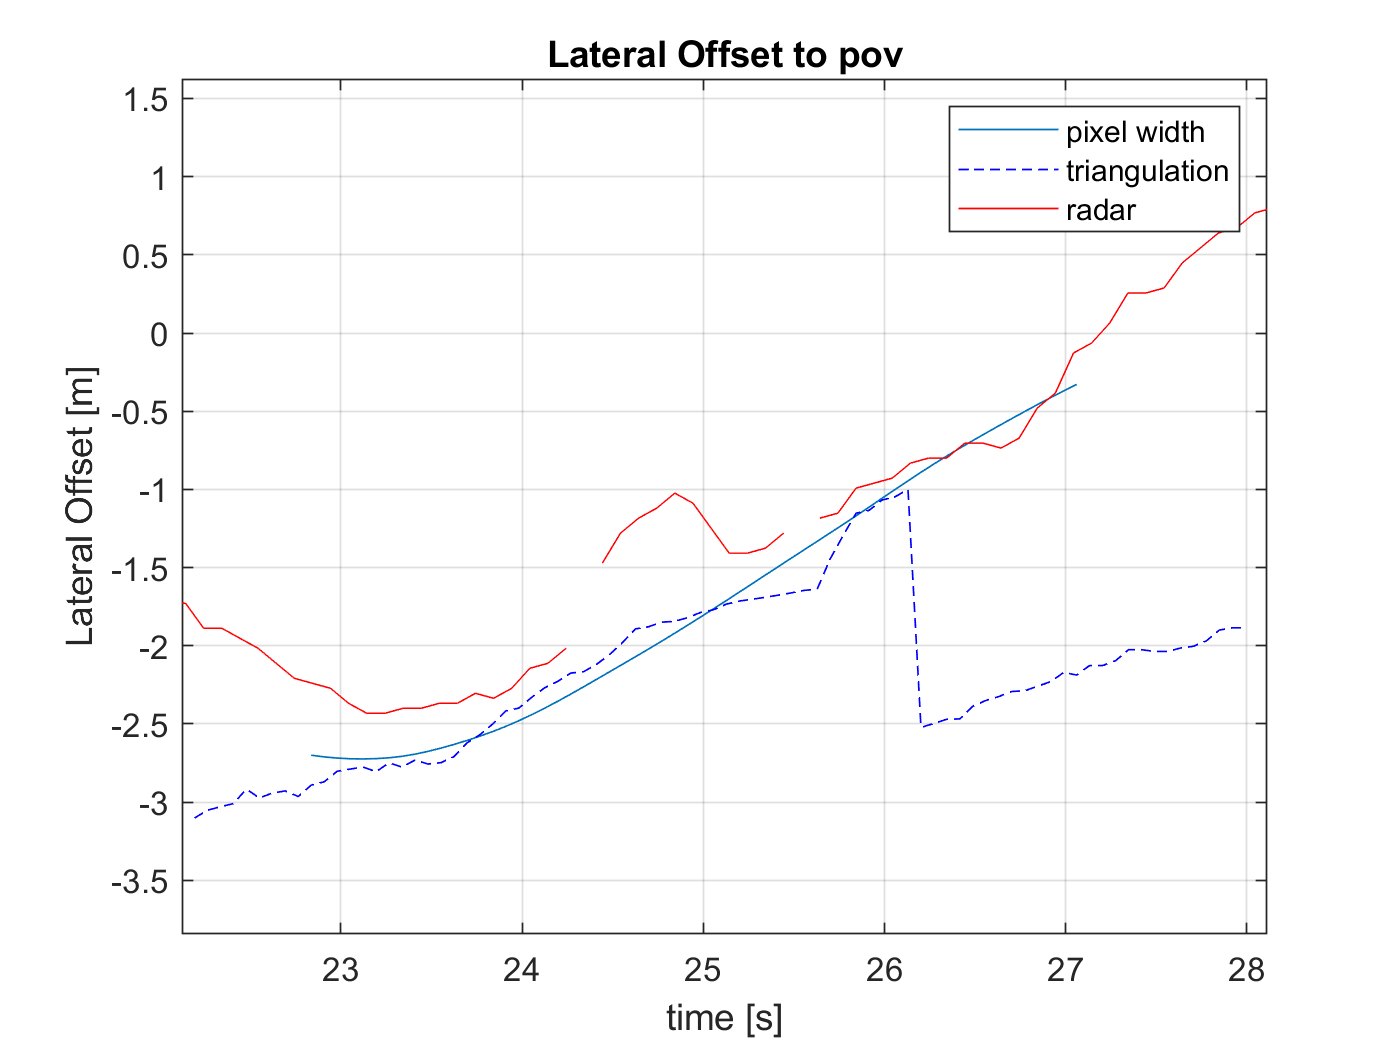
\includegraphics[width=\textwidth]{FiguresMat/homography_comparison_lat_116147345.png}
    \caption*{Event 2}
\end{minipage}
\caption{Comparing the two methods with Radar Data}
\label{fig:triangulation_comparison_latoffset}
\end{figure}

Please note that there is something wrong with the sign conversion when plotting the triangulation method in Figure \ref{fig:triangulation_comparison_latoffset}, that's why the lateral offset does the sudden jump after 26[s]. The same problem shows up in Figures \ref{fig:lat_offset_error_distance} and \ref{fig:lat_offset_error_heading}. This issue has been fixed in the tool but at the time of writing of the report (\today), the team does not have access to the updated figures. The report will be updated once the figures are acquired after the holidays.

\subsubsection{Estimation Error}

Using the radar data as reference, the error for different lateral offsets was calculated, as shown in Figure \ref{fig:lat_offset_error_distance} where it is apparent how the pixel width method remains within an error in the range $\in(-0.5, 1.5)[m]$ in event 1. In event 2, the error value is smaller, but remains within the same range. It is also apparent that the lateral offset error using the pixel width method is not affected by the actual lateral offset. On the other hand, the triangulation method shows more fluctuation when it comes to calculating the lateral offset to POV. However, this method, as discussed earlier, allows for the calculation of the lateral offset to the lane lines, and not just the relative offset between the two vehicles.

\begin{figure}[H]
\begin{minipage}[b]{0.49\textwidth}
    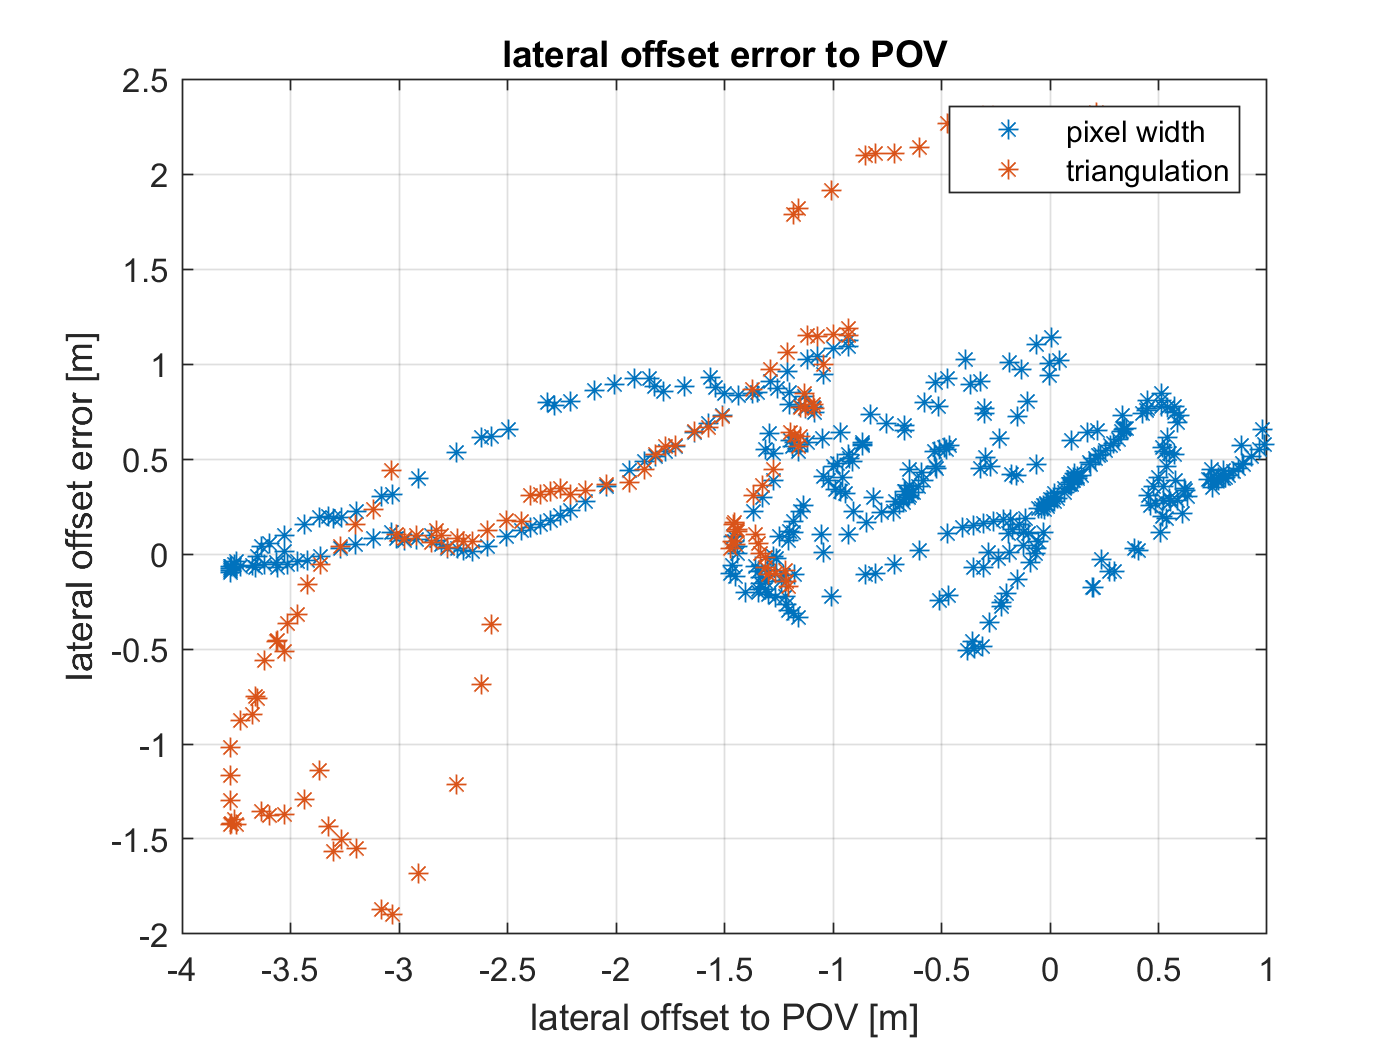
\includegraphics[width=\textwidth]{FiguresMat/range_error_lat_10794257.png}
    \caption*{Event 1}
\end{minipage}
\begin{minipage}[b]{0.50\textwidth}
    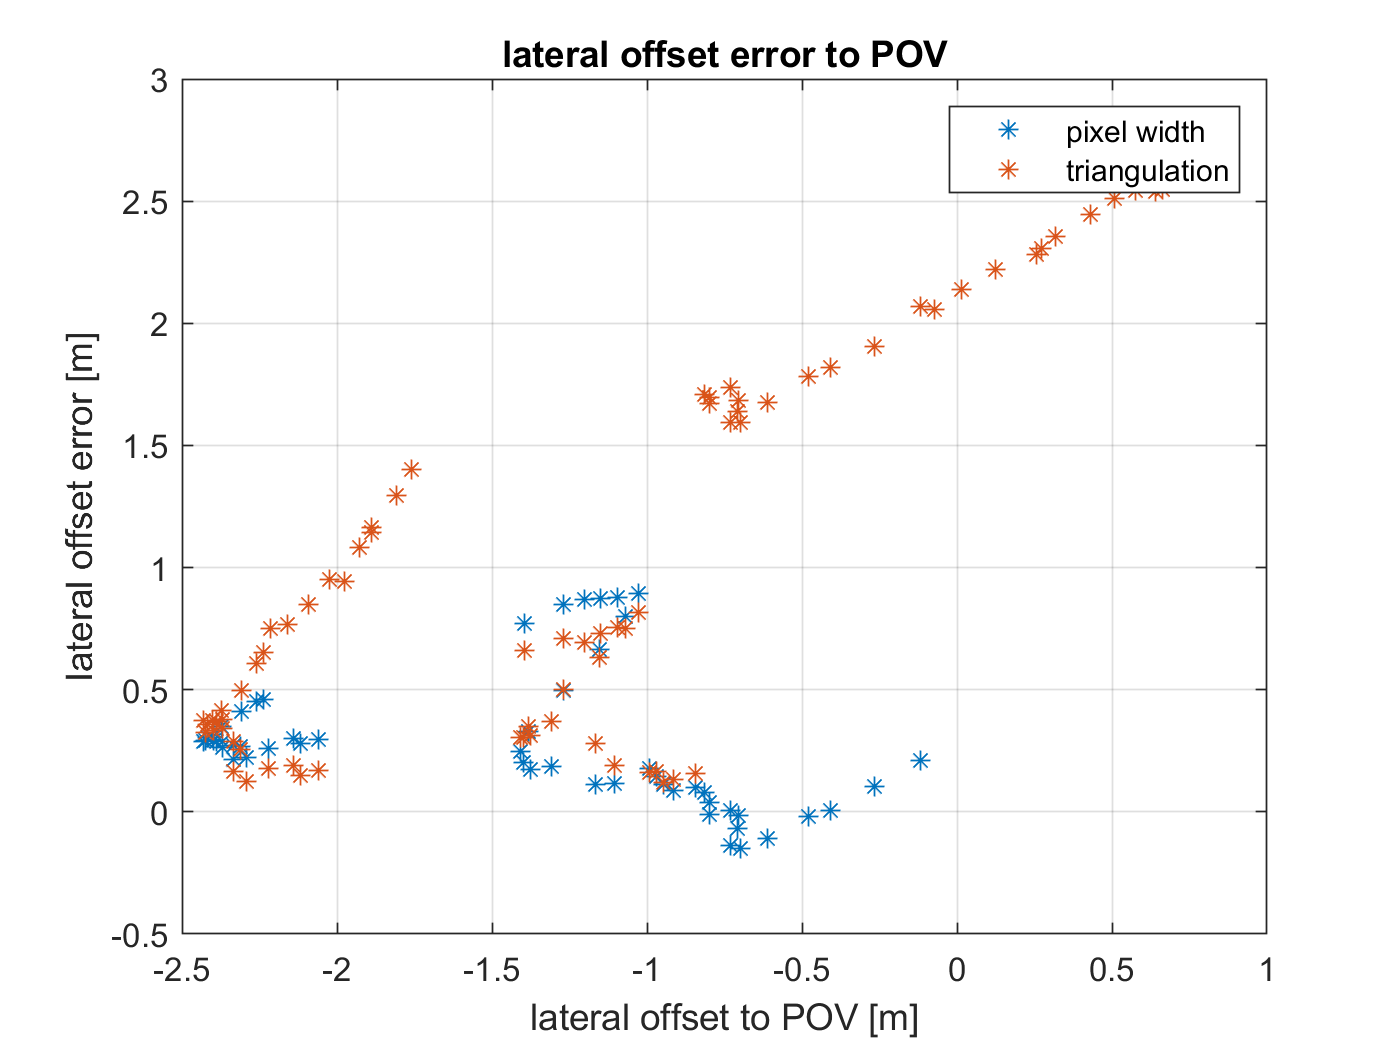
\includegraphics[width=\textwidth]{FiguresMat/range_error_lat_116147345.png}
    \caption*{Event 2}
\end{minipage}
\caption{POV lateral offset error vs POV actual lateral offset}
\label{fig:lat_offset_error_distance}
\end{figure}

This was also calculated for different heading angles, as shown in Figure \ref{fig:lat_offset_error_heading} which shows the relation between the POV's heading angle and the lateral offset estimation. From those plots, there doesn't seem to be a solid relation between the heading angle and the error in estimating the lateral offset with the pixel width method. The error seems to mostly stay in the range $\in(-0.5, 1)[m]$. The triangulation method shows a larger offset error compared to the pixel width method. Since the figure only shows two events, the results of this test are deemed to be inconclusive.

\begin{figure}[H]
\centering
\begin{minipage}[b]{0.49\textwidth}
    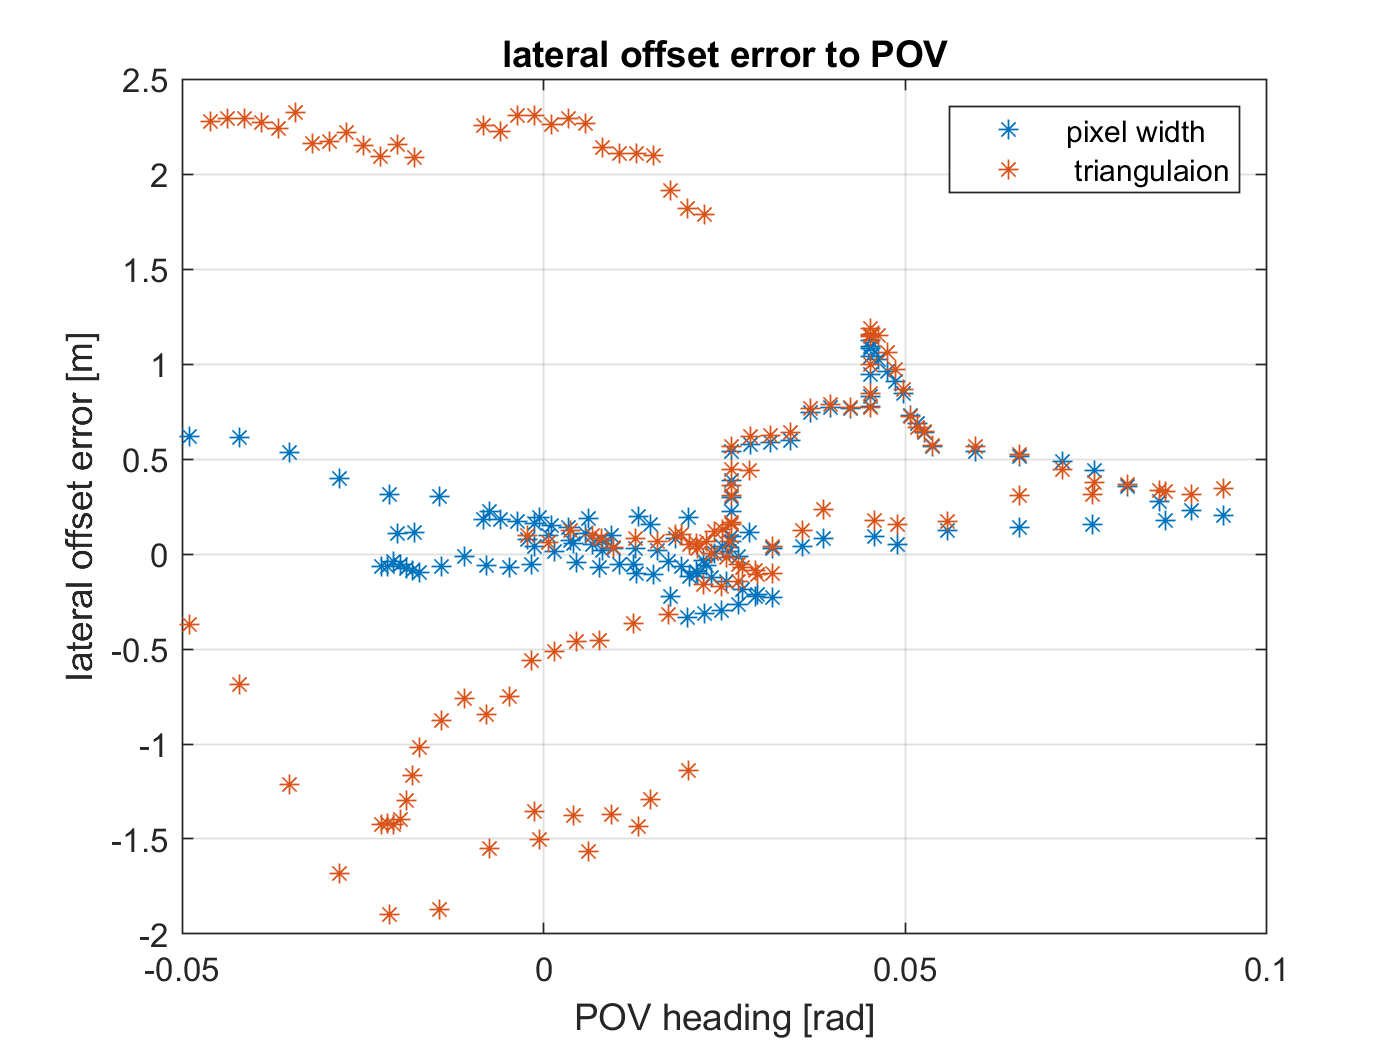
\includegraphics[width=\textwidth]{FiguresMat/range_heading_error_lat_10794257.png}
    \caption*{Event 1}
\end{minipage}
\begin{minipage}[b]{0.5\textwidth}
    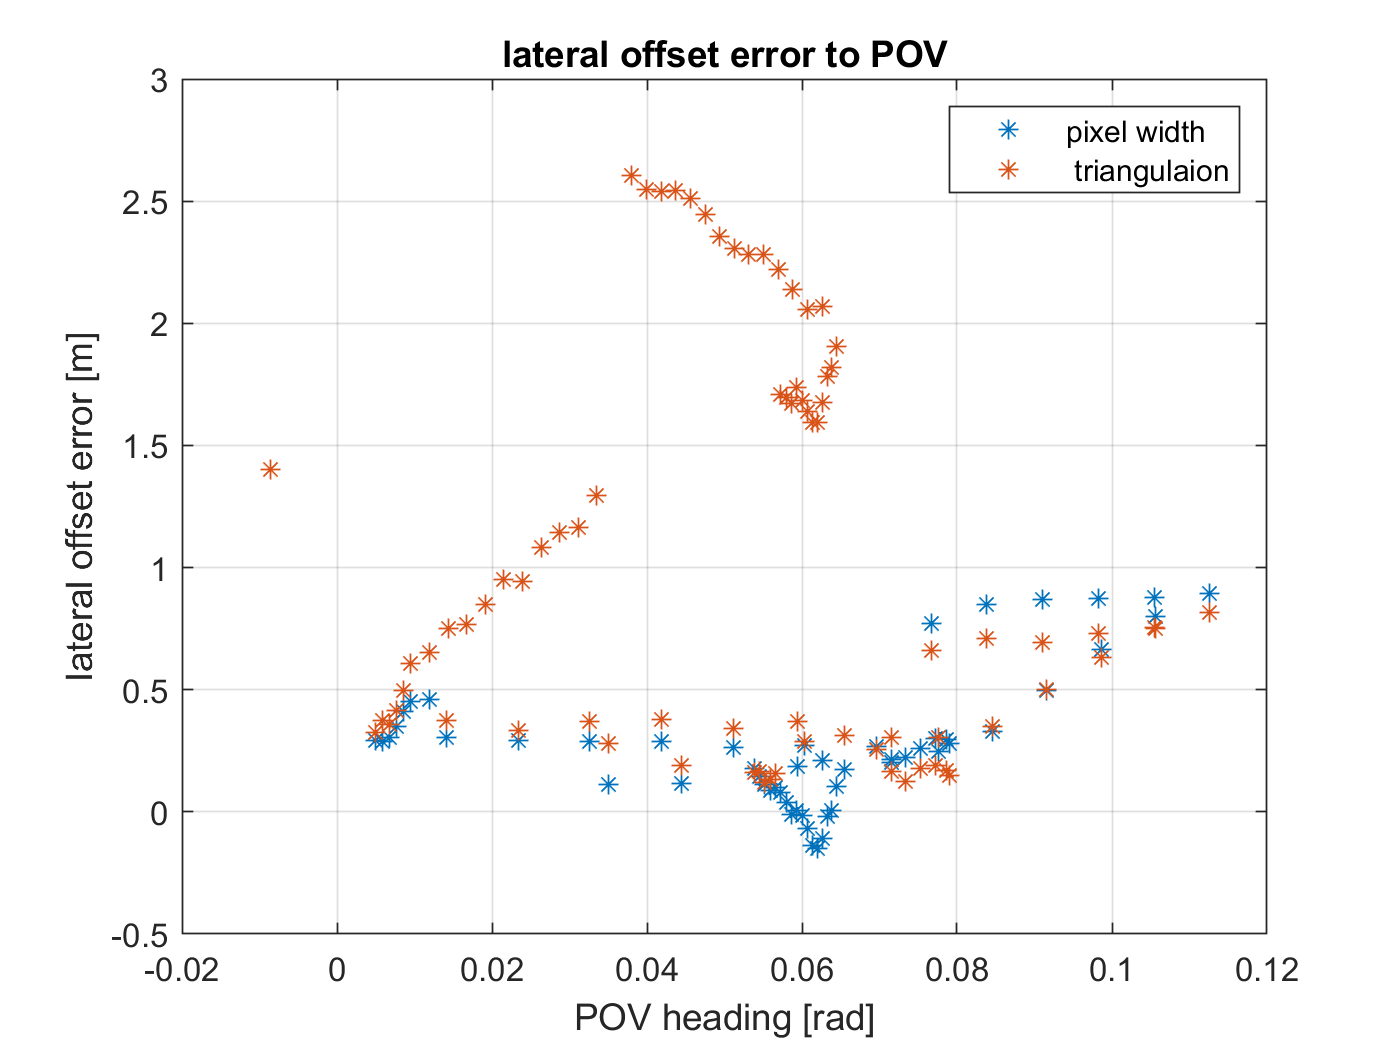
\includegraphics[width=\textwidth]{FiguresMat/range_heading_error_lat_116147345.png}
    \caption*{Event 2}
\end{minipage}
\caption{POV lat offset error vs POV estimated heading angle}
\label{fig:lat_offset_error_heading}
\end{figure}

\subsection{Range estimation}
The plots presented blow were done for critical lane-changing events in the SHRP2 data that have radar range available. These were the same as "Event 1" and "Event 2" presented earlier.  

% \subsubsection{Method 1 for Range Estimation: Pixel width}
\subsubsection{Filtering}
The estimated range acquired from the annotation tool was used to calculate the range rate to the POV. As was the case for the lateral offset, the estimated range had to be filtered to gain reasonable range rate values, as shown in Figures  \ref{fig:range_filtering_event1} and \ref{fig:range_filtering_event2}. This was done in the same was as for the lateral offset with the same filter specifications presented in Table \ref{tab:filters}.


\begin{figure}[H]
    \centering
    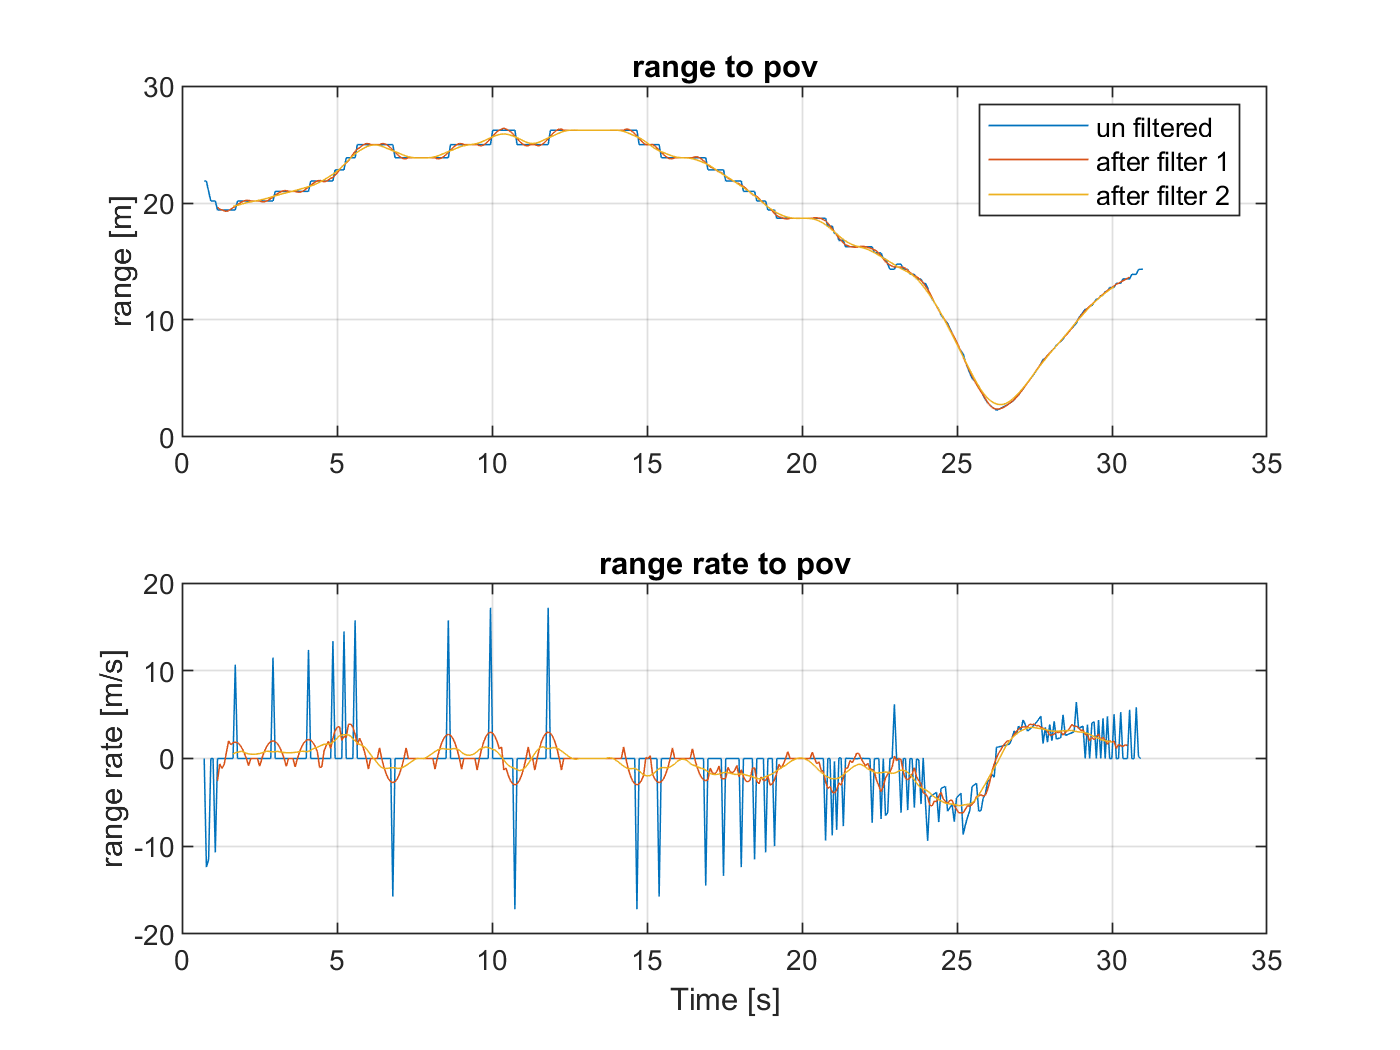
\includegraphics[width=0.8\textwidth]{FiguresMat/filter_compare_10794257.png}
    \caption{Range and Range rate with filtering Event 1}
    \label{fig:range_filtering_event1}
\end{figure}

\begin{figure}[H]
    \centering
    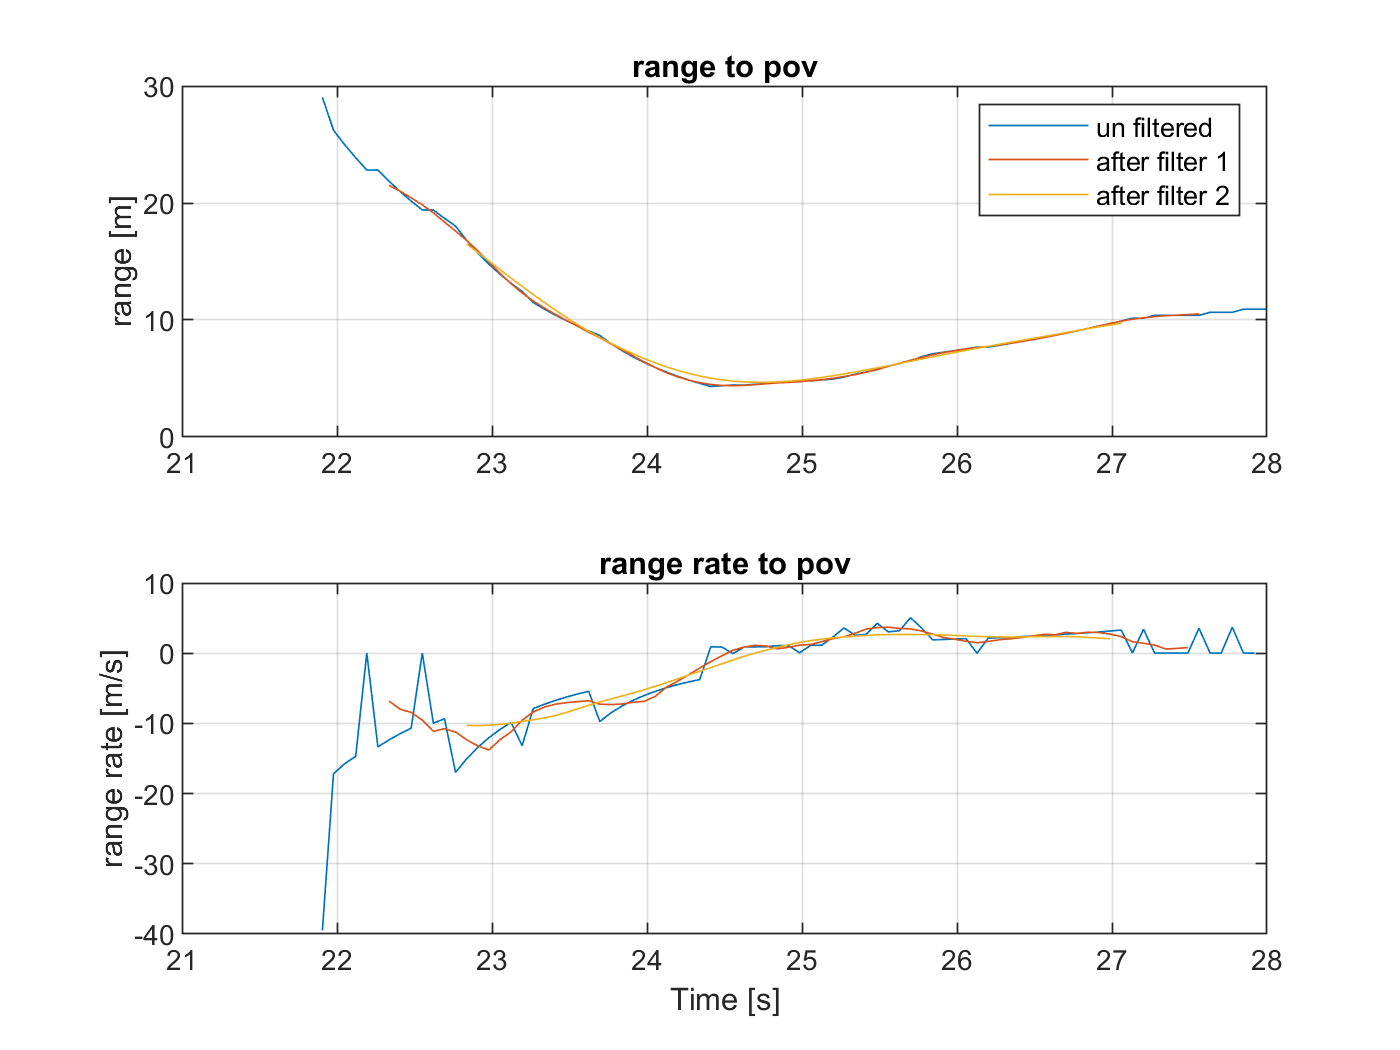
\includegraphics[width=0.8\textwidth]{FiguresMat/filter_compare_116147345.png}
    \caption{Range and Range rate with filtering Event 2}
    \label{fig:range_filtering_event2}
\end{figure}

\subsubsection{Comparing Estimated Range to Radar Data}
After filtering, the range and range rate attained from the pixel width method were compared to the radar, as shown in Figures \ref{fig:range_vs_radar_event1} and \ref{fig:range_vs_radar_event2}. From these figures, it appeared that the relative speed between the SV and the POV was higher in event 2 of Figure \ref{fig:range_vs_radar_event1} compared to event 1 of Figure \ref{fig:range_vs_radar_event2}. 

In both cases, the estimated range captured the same shape as that of the radar data. However, there appeared to be a constant offset in the range estimation in both cases, which meant that the POV seemed further away that it actually was.

\begin{figure}[H]
    \centering
    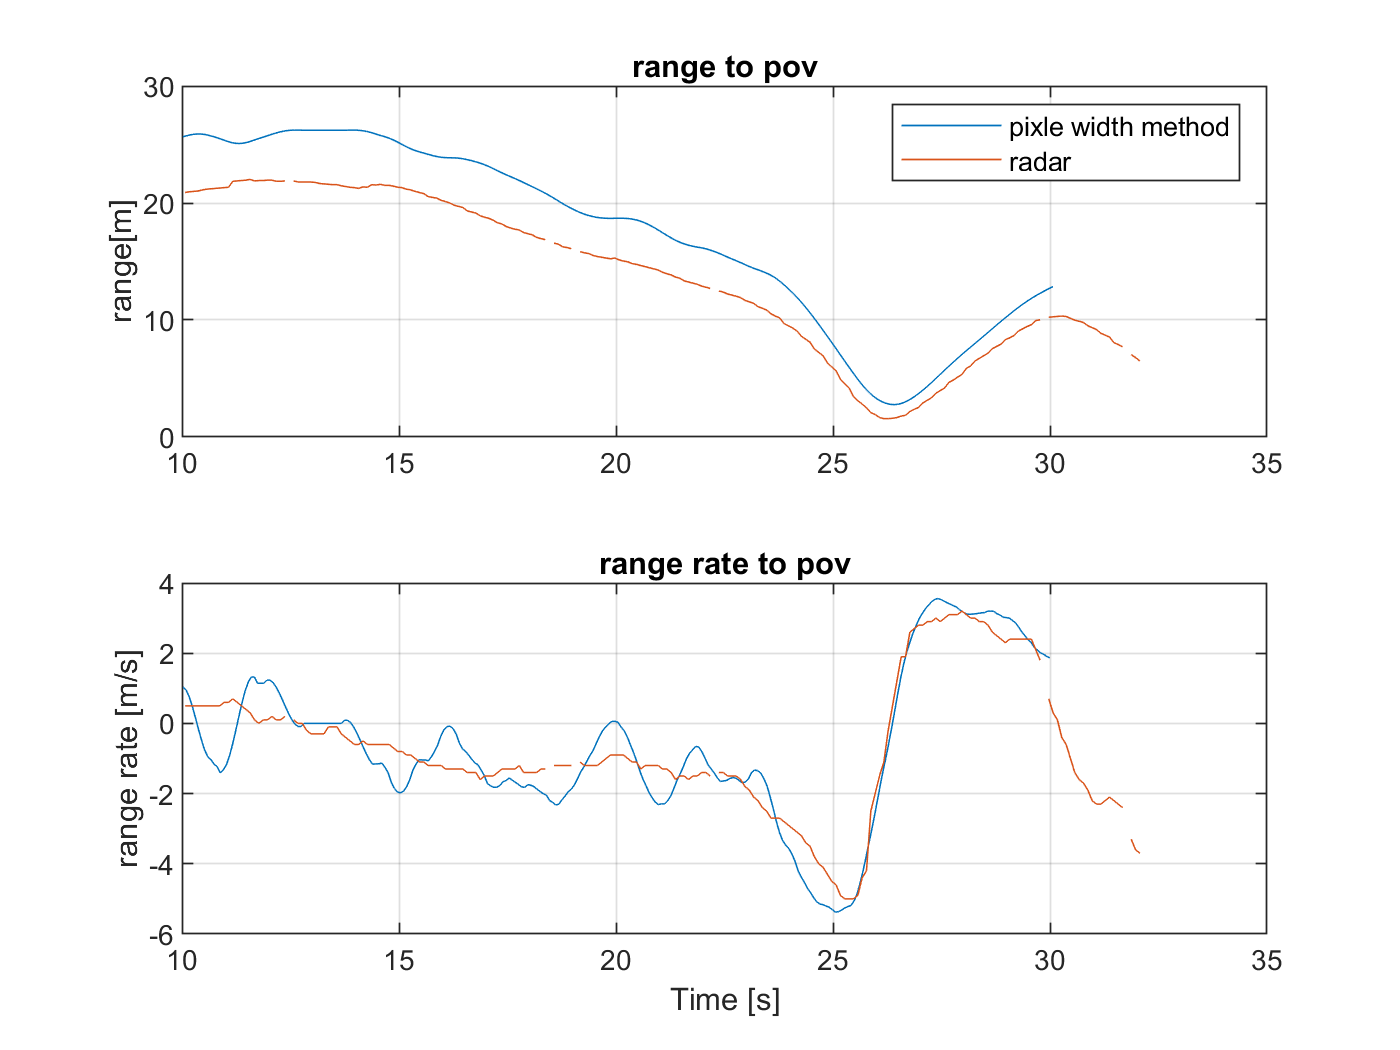
\includegraphics[width=0.8\textwidth]{FiguresMat/radar_compare_10794257.png}
    \caption{Estimated Range vs Radar Data Event 1}
    \label{fig:range_vs_radar_event1}
\end{figure}

\begin{figure}[H]
    \centering
    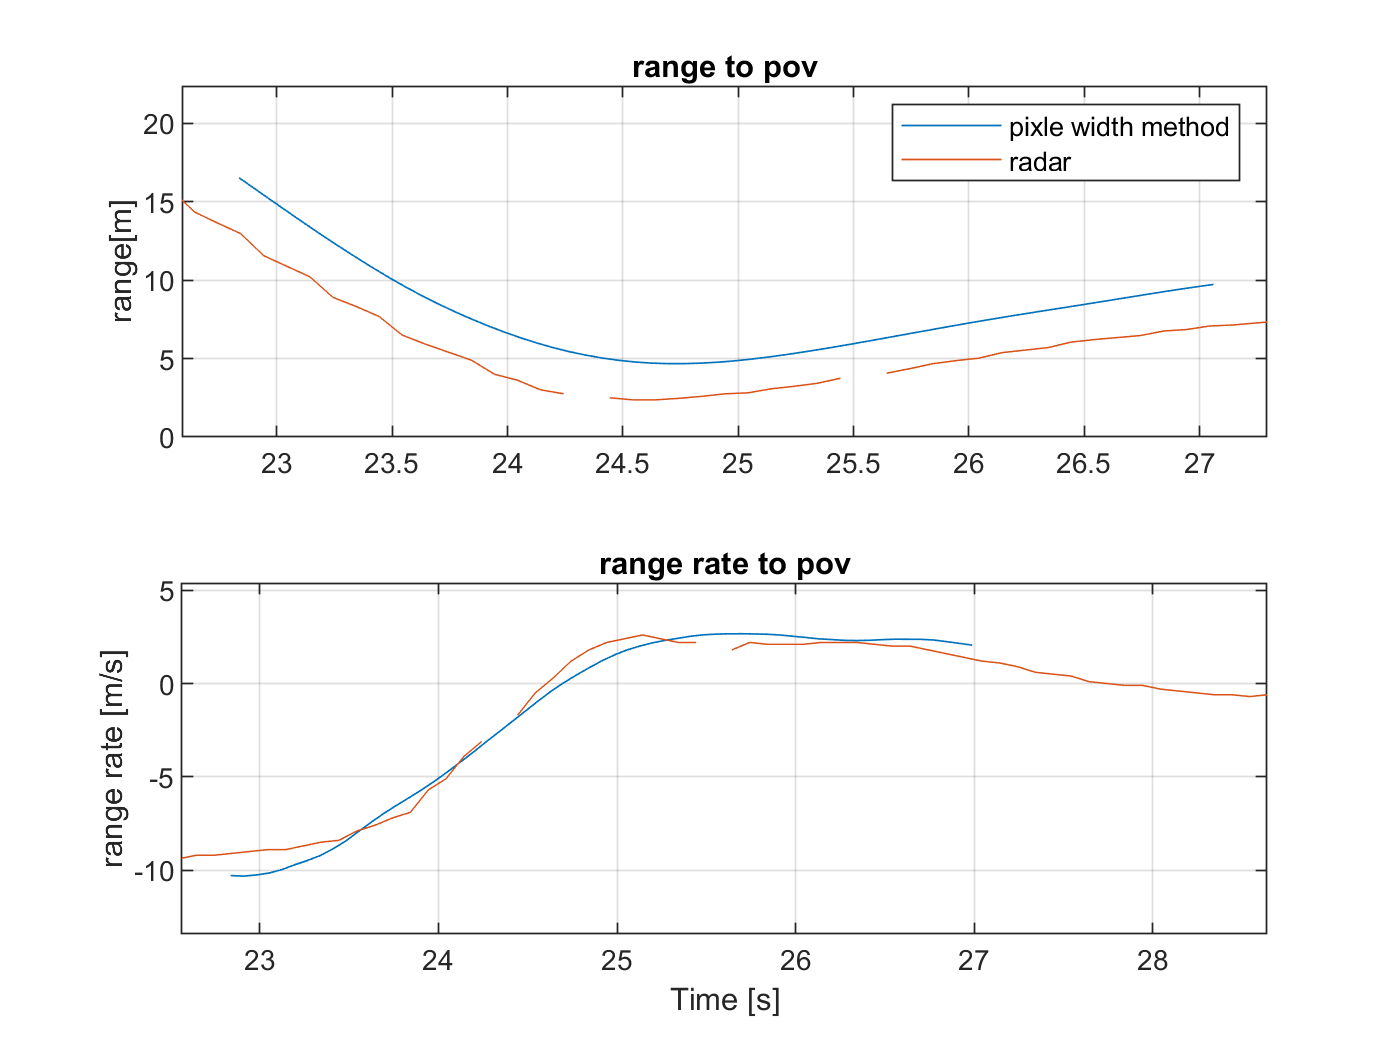
\includegraphics[width=0.8\textwidth]{FiguresMat/radar_compare_116147345.png}
    \caption{Estimated Range vs Radar Data Event 2}
    \label{fig:range_vs_radar_event2}
\end{figure}



For event 1 of Figure \ref{fig:range_vs_radar_event1}, the range rate fluctuated for ranges above $\approx 15[m]$. At closer ranges below $\approx 15[m]$, the range rate error was smaller and appeared to keep the same shape and value as that of the radar data. 

For event 2 of Figure \ref{fig:range_vs_radar_event2}, tracking was started when the POV was at a range of $\approx 15[m]$ and, as a result, both the range and range rate did not fluctuate.

\subsubsection{Comparing Triangulation method to Pixel Width method and Radar Data}

The triangulation method is also tested for the range estimation and compared to the radar data as shown in Figure \ref{fig:triangulation_comparison_range}. It is evident from the figure that the triangulation method offers more accurate results compared to the pixel width method, but shows more fluctuation. Upon further testing on several events, it was proven that although the triangulation method might provide a more accurate result at some times, the pixel width method has a better precision where the results would be relatively consistent. One should keep in mind also that the fluctuation shown in Event 1 of Figure \ref{fig:triangulation_comparison_range} is caused by the SV changing lanes on a curved road as mentioned earlier.


\begin{figure}[H]
\begin{minipage}[b]{0.49\textwidth}
    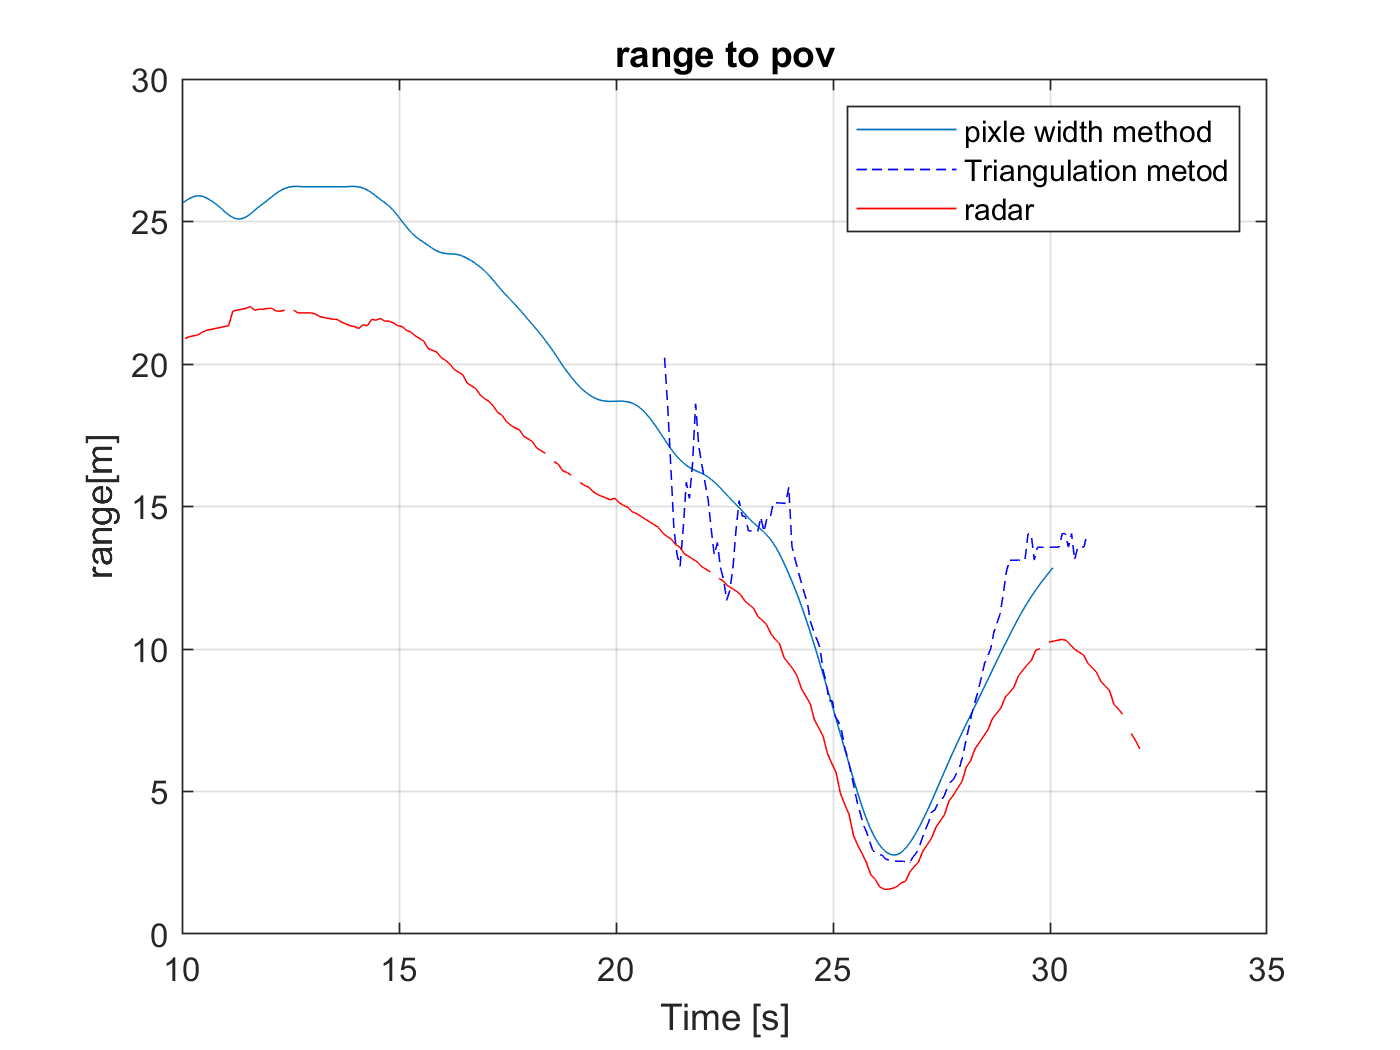
\includegraphics[width=\textwidth]{FiguresMat/homography_compare_long_10794257.png}
    \caption*{Event 1}
\end{minipage}
\begin{minipage}[b]{0.50\textwidth}
    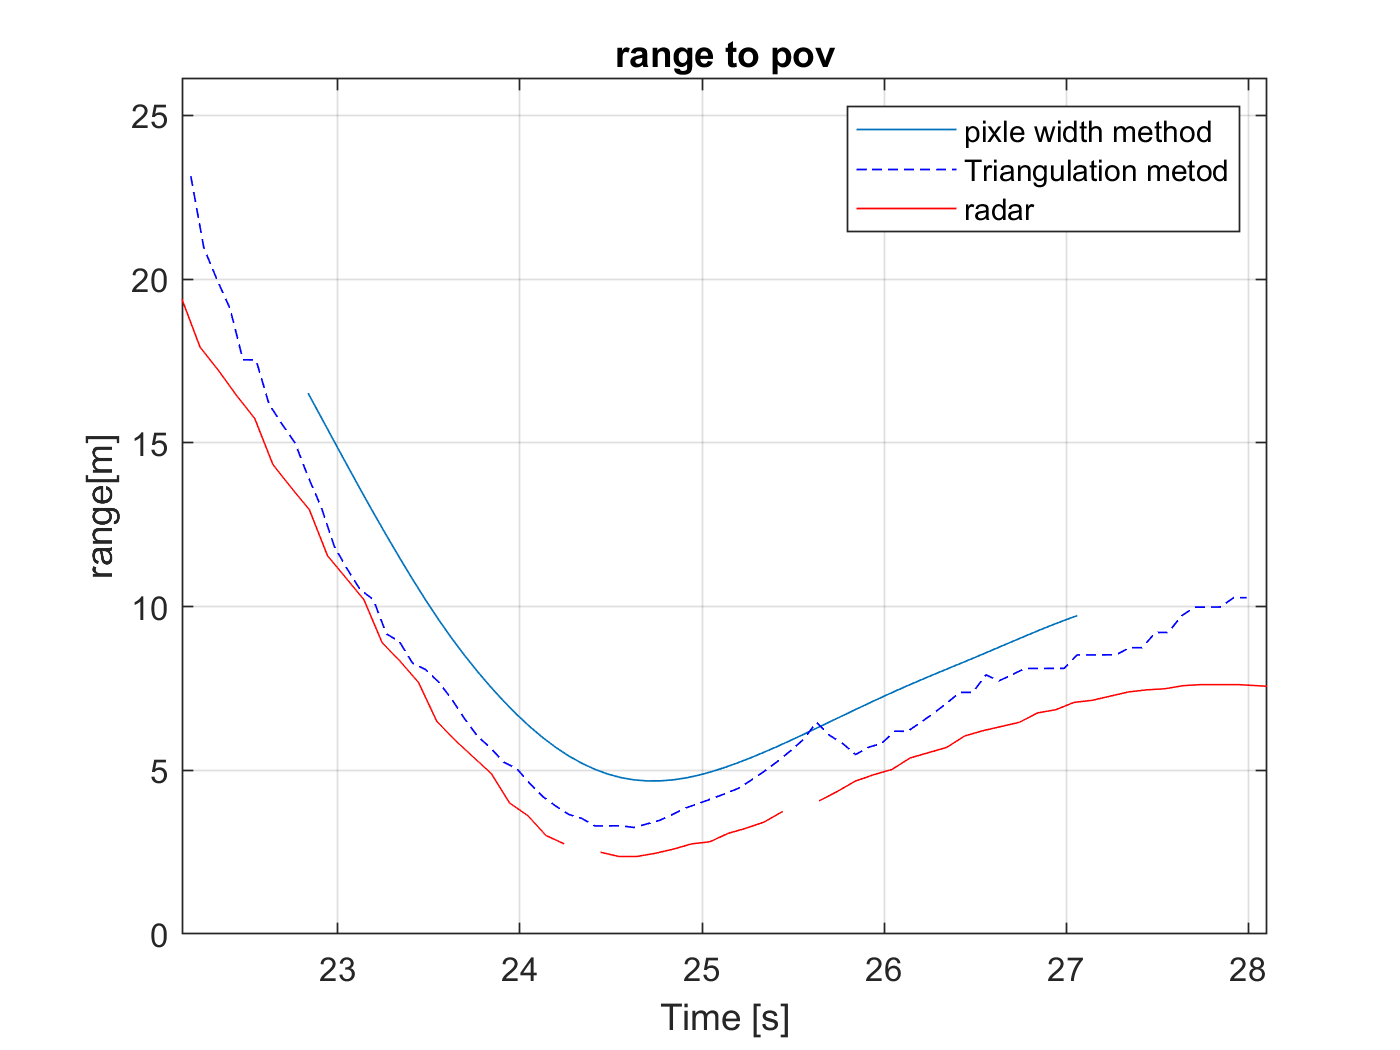
\includegraphics[width=\textwidth]{FiguresMat/homography_compare_long_116147345.png}
    \caption*{Event 2}
\end{minipage}
\caption{Comparing the two methods with Radar Data}
\label{fig:triangulation_comparison_range}
\end{figure}

\subsubsection{Estimation Error}

To understand the performance of the two methods in estimating the range between the SV and POV, some figures were developed that show the relation between the range and its error (Figure \ref{fig:range_error_vs_radar}) as well as the relation between the range and the POV heading angle (Figure \ref{fig:range_error_vs_heading}). 

From Figure \ref{fig:range_error_vs_radar}, three main characteristics are observed. First, and most importantly, both methods show that as the range increases, the error increases. Second, the triangulation method has a lower error on average compared to the pixel width method. Third, the triangulation method has more fluctuation while the pixel width method seems to give more stable ranges. Fourth, at higher ranges there is more fluctuation in the error for both methods.

\begin{figure}[H]
\begin{minipage}[b]{0.49\textwidth}
    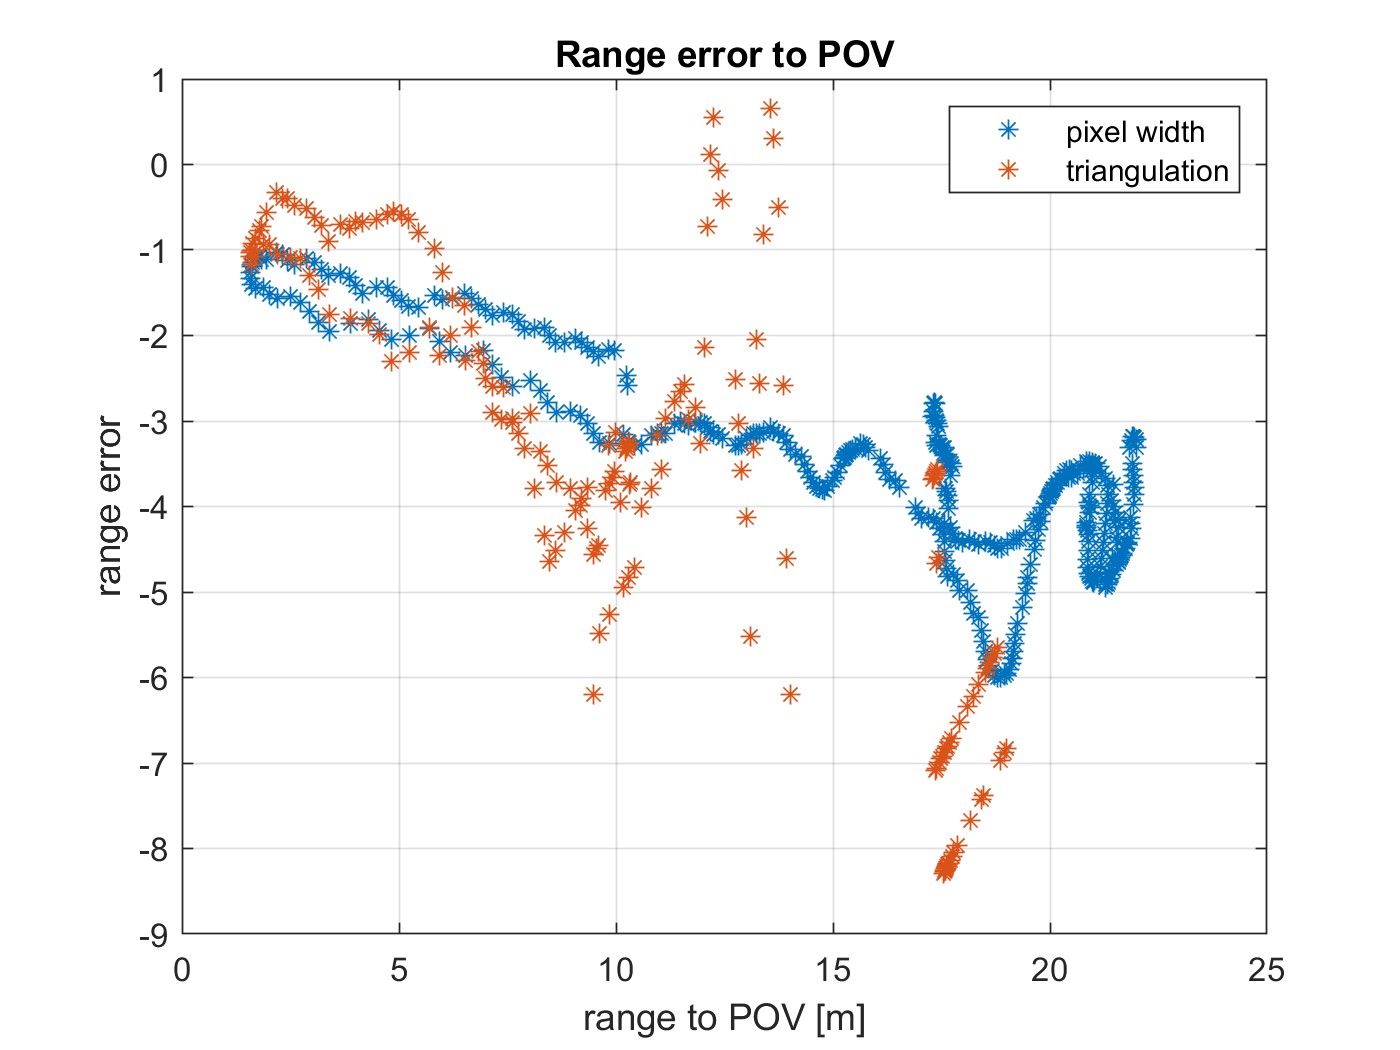
\includegraphics[width=\textwidth]{FiguresMat/range_error_long_10794257.png}
    \caption*{Event 1}
\end{minipage}
\begin{minipage}[b]{0.50\textwidth}
    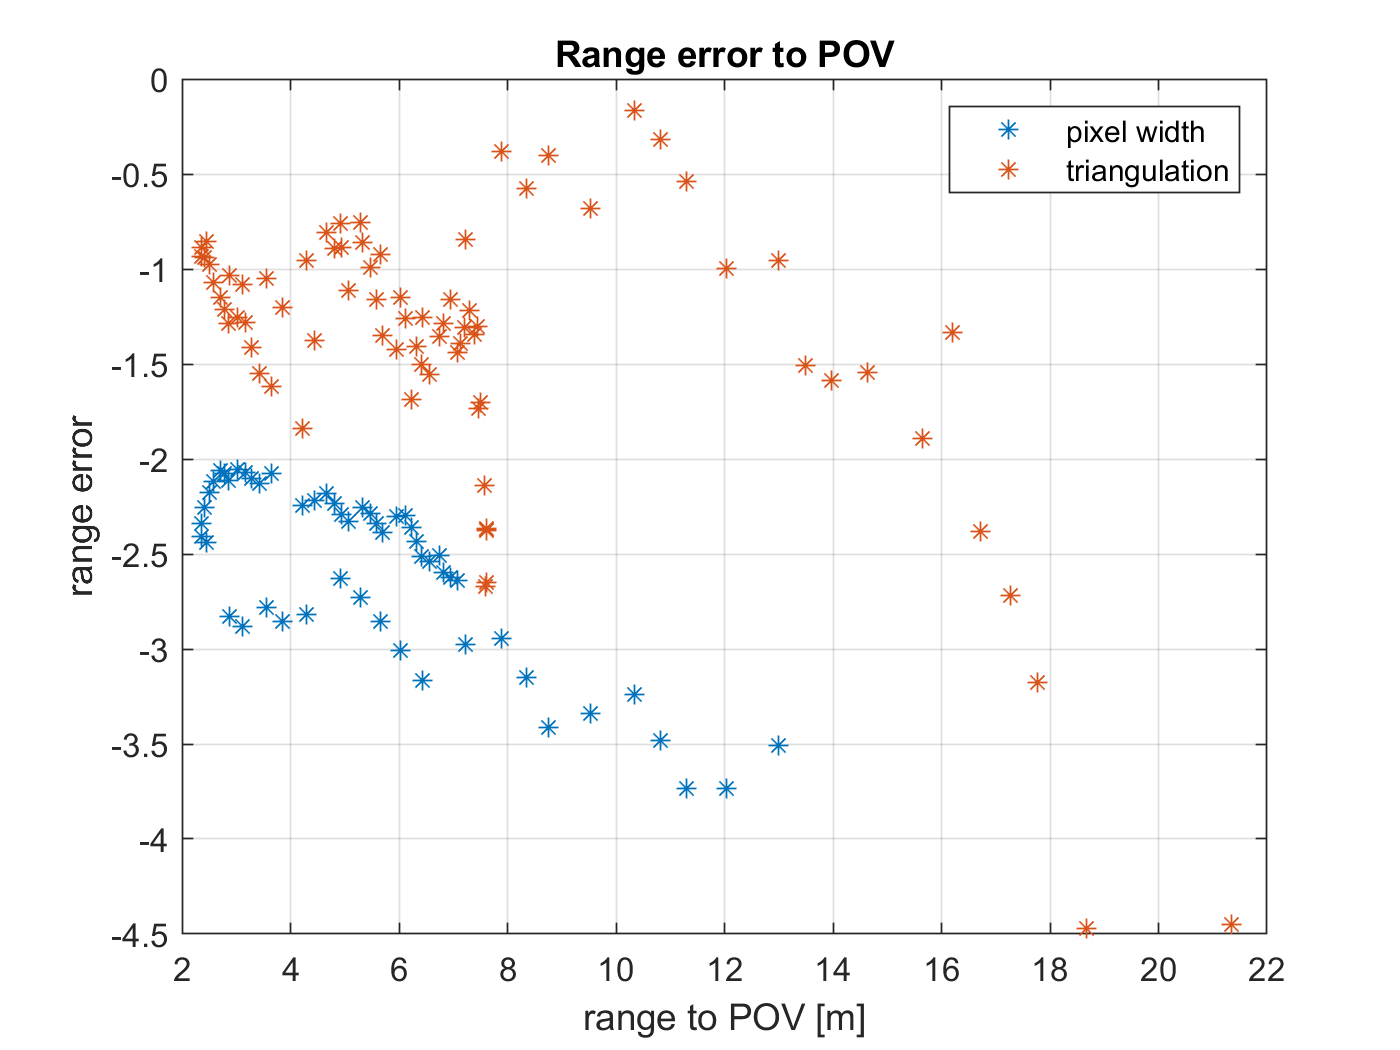
\includegraphics[width=\textwidth]{FiguresMat/range_error_long_116147345.png}
    \caption*{Event 2}
\end{minipage}
\caption{POV range error vs POV actual range}
\label{fig:range_error_vs_radar}
\end{figure}

From Figure \ref{fig:range_error_vs_heading}, not much can be seen. The results are similar to what was discussed above where the triangulation method is more accurate but less precise compare to the pixel width method. Interestingly, it can be seen from Event 2 of Figure \ref{fig:range_error_vs_heading} that as the heading angle increases, the range error decreases. This is more apparent in the pixel width method.

\begin{figure}[H]
\begin{minipage}[b]{0.49\textwidth}
    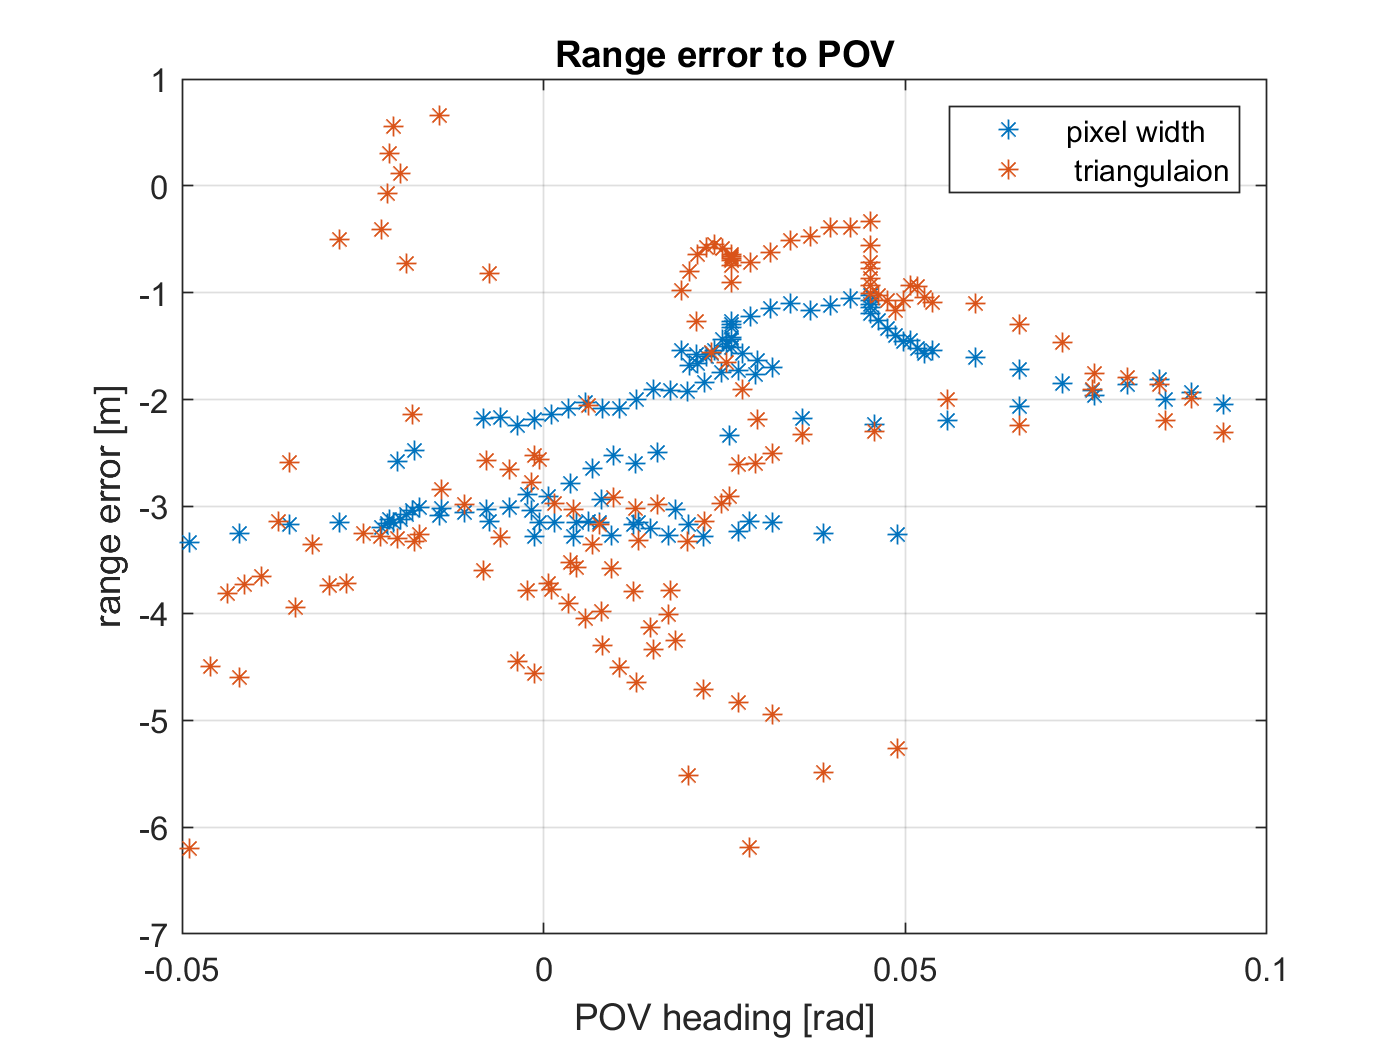
\includegraphics[width=\textwidth]{FiguresMat/range_heading_error_long_10794257.png}
    \caption*{Event 1}
\end{minipage}
\begin{minipage}[b]{0.50\textwidth}
    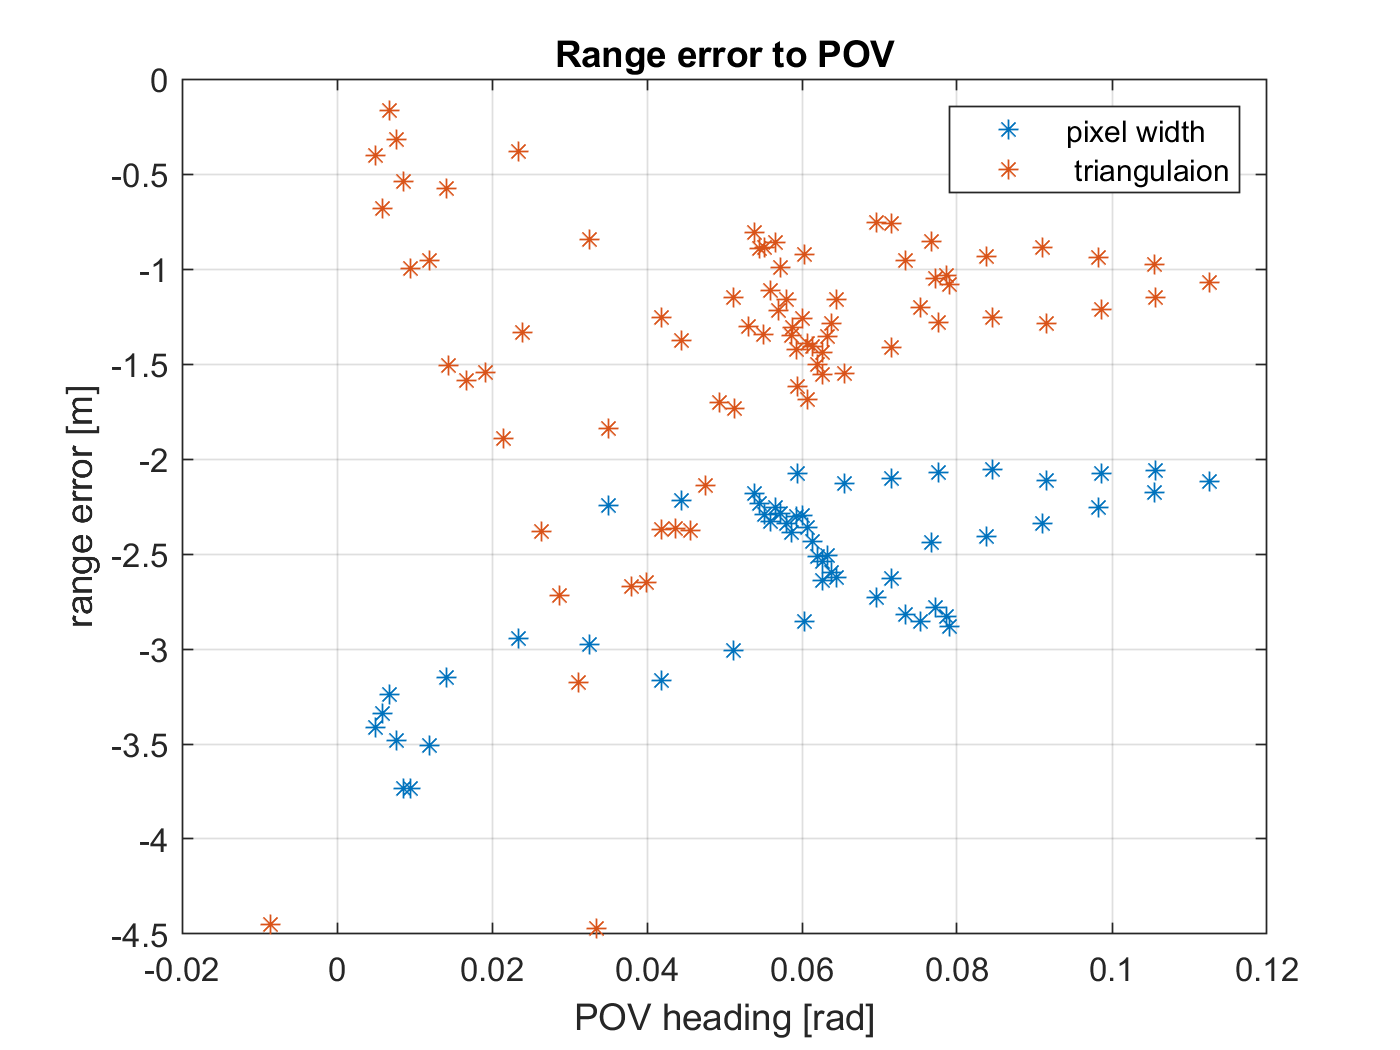
\includegraphics[width=\textwidth]{FiguresMat/range_heading_error_long_116147345.png}
    \caption*{Event 2}
\end{minipage}
\caption{POV range error vs POV estimated heading}
\label{fig:range_error_vs_heading}
\end{figure}

\subsection{Vehicle tracking}
The three methods of tracking that were previously mentioned were studied during the course of project. Due to the time frame of the project, more focus was put on manual annotation, since it was the easiest to implement and was needed for testing other functions in the tool, such as range estimation. Automatic tracking was studied briefly, but was not implemented in the final tool. The results from all there methods are presented below. 

\subsubsection{Manual Tracking}

It was found that this method, although simple, did help identify the POV accurately given the relative speed between the POV and the SV was constant and both vehicles are heading in the same direction, as shown in Figure \ref{fig:POV_tracking_interpolation}, where the user inputs the POV placement in frames 1 and 30, and the tool interpolated the placement in the frames between. In this case, the user was able to track the vehicle in 30 frames through manually defining the POV in only 2 frames. 

\begin{figure}[H]
\centering
\captionsetup{justification=centering}
\begin{minipage}[b]{0.45\linewidth}
    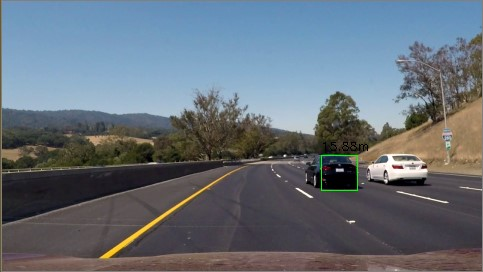
\includegraphics[width=\linewidth]{Figures/interpolation_frame_0.jpg}
    \caption*{User input\\ frame 1 (Green)}
\end{minipage}
\begin{minipage}[b]{0.45\linewidth}
    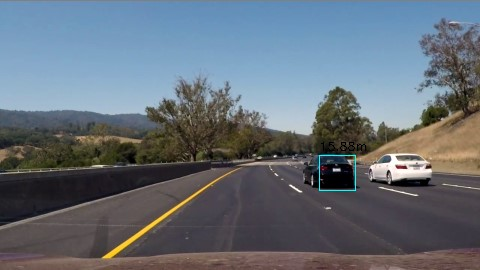
\includegraphics[width=\linewidth]{Figures/interpolation_frame_10.jpg}
    \caption*{Interpolated POV placement\\ frame 10 (Aqua)}
\end{minipage}
\vspace{5mm}\\
\begin{minipage}[b]{0.45\linewidth}
    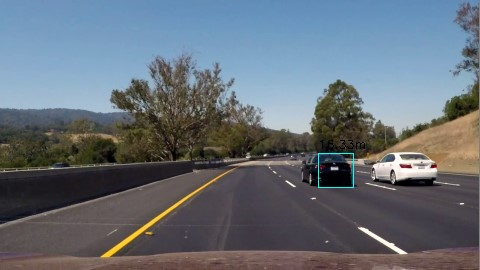
\includegraphics[width=\linewidth]{Figures/interpolation_frame_20.jpg}
    \caption*{Interpolated POV placement\\ frame 20 (Aqua)}
\end{minipage}
\begin{minipage}[b]{0.45\linewidth}
    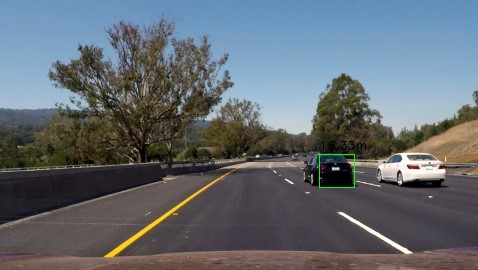
\includegraphics[width=\linewidth]{Figures/interpolation_frame_30.jpg}
    \caption*{User input\\ frame 30 (Green)}
\end{minipage}
\caption{Results from the interpolation method for vehicle tracking}
\label{fig:POV_tracking_interpolation}
\end{figure}

This method becomes less accurate in transient maneuvers, where the relative speed between the vehicles is not constant, i.e the vehicles are braking or accelerating. What this means is that the user would need to annotate more frames for the POV tracking to be more accurate. 

\subsubsection{Automatic and Semi-automatic Vehicle Tracking}
\label{sec:3.6.2}
Automatic vehicle detection was achieved on single images using openCV and a pre-trained neural network called You Only Look Once (YOLO) which is an advanced tool developed for object detection\cite{Redmon_2016_CVPR}, as seen in Figure \ref{fig:yolo_image}.

\begin{figure}[H]
    \centering
    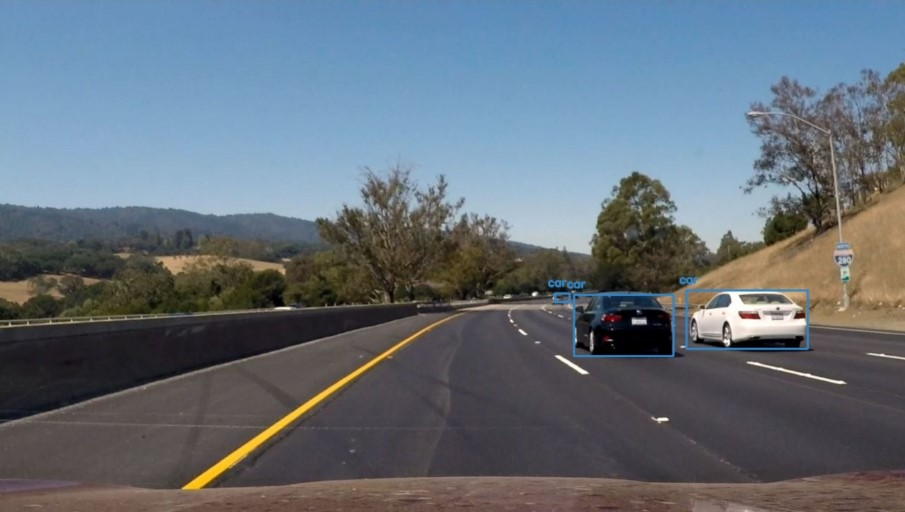
\includegraphics[width=\textwidth]{Figures/yolo_image.jpg}
    \caption{Vehicle detection with the YOLO algorithm}
    \label{fig:yolo_image}
\end{figure}

As seen in the Figure \ref{fig:yolo_image}, YOLO is able to detect the entire vehicle. This is a problem since the method used for range estimation in this project requires only the placement of the rear of the vehicle in the image. This meant that the bounding box marked by YOLO is not on its own usable for range estimation. Instead it would have to be combined with some user defined box around the rear of the vehicle, which would make the tracking semi-automatic. Due to the limited time of this project, this method was not tested.


\subsection{Tool and Graphical User Interface design}

The design of the GUI was kept simple as initially intended, following the same outline described in the methodology section. More focus was put on verifying that the user inputs were processed and used correctly within the program to extract relevant variables. 

\subsubsection{Video player and Controls}

Upon initialization, the user is asked to choose the path of the video that is to be annotated. The user shall then have the option to either re-annotate the data using previously annotated data for the same video, or start over. The video will then be loaded and the user presented with the view shown in  Figure \ref{fig:GUI_overview}.

\begin{figure}[H]
\begin{tikzpicture}
    \node[anchor=south west,inner sep=0] at (0,0) {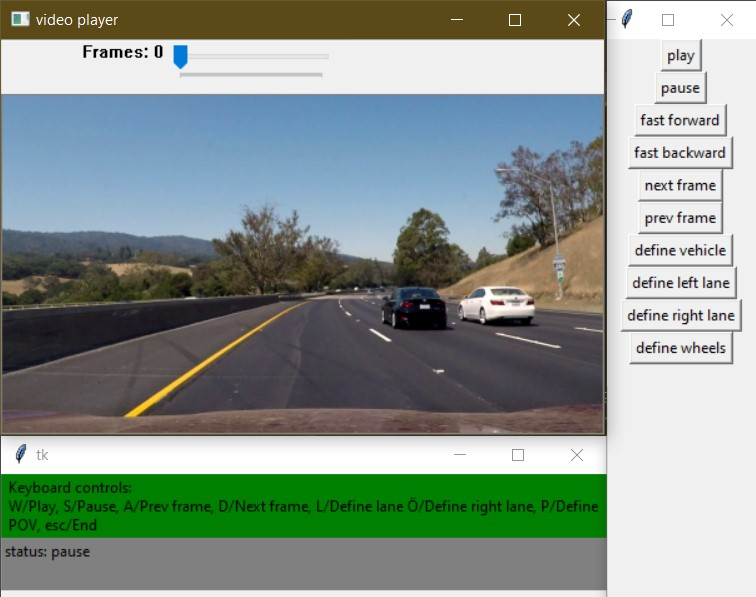
\includegraphics[width=\textwidth]{Figures/GUI_windoe.jpg}};
    \draw[red,ultra thick,rounded corners] (16,0) rectangle (12.9,12.8) node[above right] {Control button window};
    \draw[green,ultra thick,rounded corners] (12.8,3.4) rectangle  (-0.1,12.8) node[above right] {Main window for video player};
    \draw[blue,ultra thick,rounded corners] (12.8,3.3) rectangle  (-0.1, -0.1) node[below right] {Information window};
\end{tikzpicture}
\caption{Overview of GUI}
\label{fig:GUI_overview}
\end{figure}

\subsubsection{Displaying Information}

% To allow the user to identify how inputs were interpreted by the program, different colors were used to display this information in the main window. Below is a description of how this was achieved. 

% Moreover, a the information window provides information on the current status of the program and what the user should do next.



When a user chooses to input the  placement of different objects in the image, the information window will show what the user has chosen to specify. When the user is defining an object, the figures drawn in the main window are blue, stating the the user is still editing this specific input. When the user presses enter, the input is confirmed and drawn with a different color. These stages are shown in Figure \ref{fig:stages_of_inputs} below. 


\begin{figure}[H]
\centering
\begin{minipage}[b]{0.45\linewidth}
    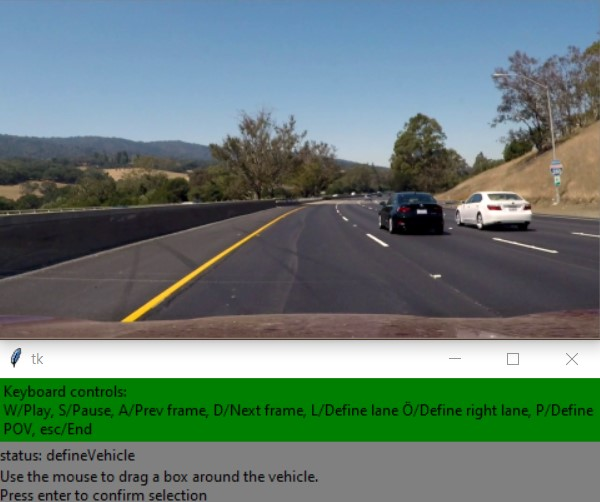
\includegraphics[width=\textwidth]{Figures/define_vehicle_1.jpg}
    \caption*{User pressed define POV button}
\end{minipage}
\begin{minipage}[b]{0.45\linewidth}
    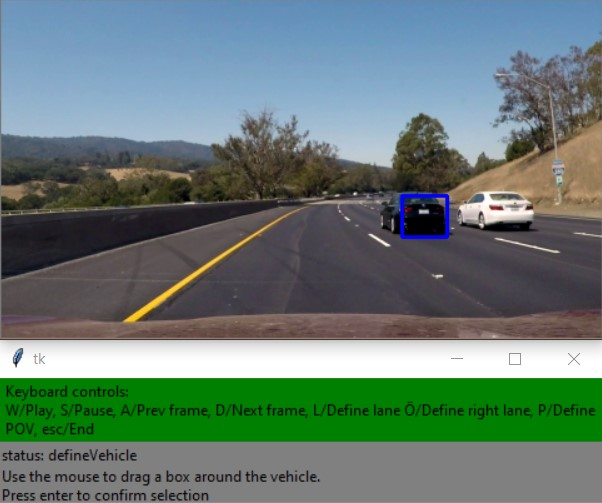
\includegraphics[width=\textwidth]{Figures/define_vehicle_2.jpg}
    \caption*{User is defining POV (Blue)}
\end{minipage}
\vspace{5mm}\\
\begin{minipage}[b]{0.45\linewidth}
    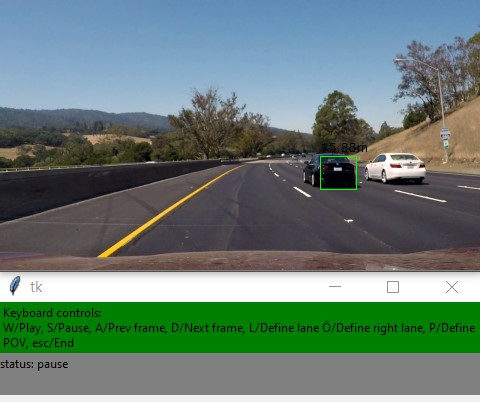
\includegraphics[width=\textwidth]{Figures/define_vehicle_3.jpg}
    \caption*{User has confirmed the input (Green)}
\end{minipage}
\caption{The different stages of taking user inputs}
\label{fig:stages_of_inputs}
\end{figure}

The same was done for all four input types using blue when the user is editing an input and a different colour when the user has confirmed the input, as seen in 
Figure \ref{fig:define_all}. Moreover, the colour of an interpolated placement is shown in a different colour to help the user know what is user defined and what is interpolated, as seen in Figure \ref{fig:POV_tracking_interpolation}. 

\begin{figure}[H]
    \centering
    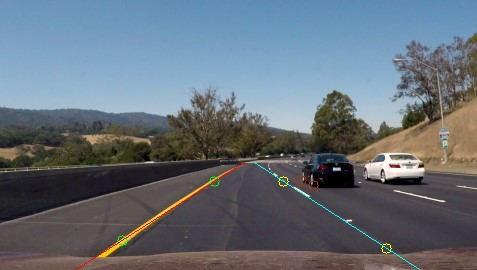
\includegraphics[width=\textwidth]{Figures/define_all.jpg}
    \caption{Different colours used for Left lane, Right lane and POV wheels}
    \label{fig:define_all}
\end{figure}

Also, two plots are made in real time as the user is inputting data, as seen in Figure \ref{fig:online_plots}. The first plot shows the calculated range and range rate to the POV. This plot will also plot radar data if that is available. The second plot uses the distances gained from the triangulation method to draw the area around the SV as seen from above. This was especially helpful during the development stage, where these plots helped visualise the output parameters from the tool, such as range, lateral offset and heading angle. 

\begin{figure}[H]
\centering
\begin{minipage}[b]{0.45\linewidth}
    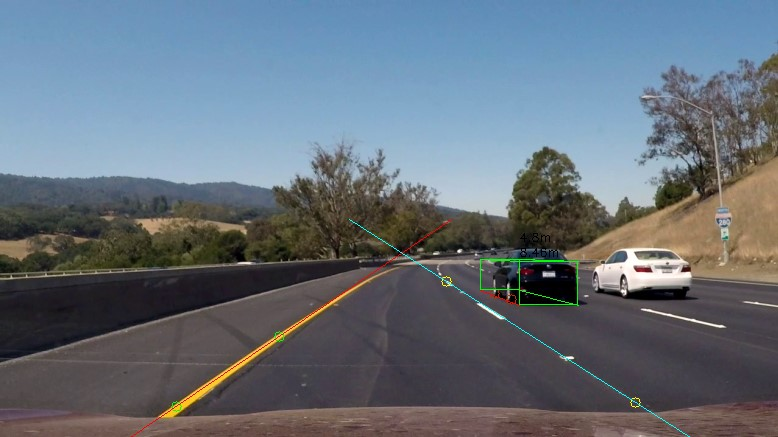
\includegraphics[width=\textwidth]{Figures/GUI_all_inputs.jpg}
    \vspace{2mm}
    \caption*{View in the main window}
\end{minipage}
\begin{minipage}[b]{0.45\linewidth}
    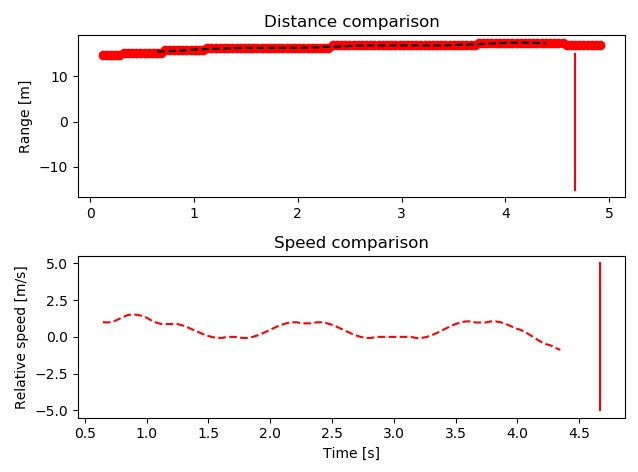
\includegraphics[width=\textwidth]{Figures/online_plot.jpg}
    \caption*{Real-time plot of range and range rate to POV}
\end{minipage}
\begin{minipage}[b]{0.45\linewidth}
    \includegraphics[width=\textwidth]{Figures/GUI_all_inputs_2d.jpg}
    \caption*{Top view plot}
\end{minipage}
\caption{Overview of the different plots}
\label{fig:online_plots}
\end{figure}


\subsubsection{Loading and Saving User Inputs}

Upon selecting a video to annotate, the program will find the event ID from the video name and search in a specified folder for the $.mat$ file containing the time-series data for the SV provided in the SHRP2 data. If no file is found, a message will be printed stating this, but the user will be able to annotate the video nonetheless.

As mentioned in section \ref{sec:Loading_and_saving_data}, two output files are created upon finishing the annotation, one $.mat$ file and on $.pickle$ file, both containing the same data. The $.pickle$ file allows for easier re-annotation of a previously annotated video. Upon selecting a video, the program will search for a $.pickle$ file with the same event ID. If one is found, the user will have the option to either reuse the old annotation and modify it, or start an new annotation.  

\subsubsection{Testing User Sensitivity}

To test the sensitivity of the tool for different annotations, one video was annotated 5 times by the same user, as seen in Figure \ref{fig:same_vid_5times}. The average for all 5 annotations has been computed and compared to the radar range, as seen in Figure \ref{fig:average_vs_radar}.

Initially, this was supposed to be done by all four members of the team. however, due to time constraints, only one member had the time to conduct this test. This was done for Event 1.

\begin{figure}[H]
    \centering
    \includegraphics[width=\textwidth]{Figures/user_comparison.jpg}
    \caption{Same video annotated 5 times by same user}
    \label{fig:same_vid_5times}
\end{figure}

As seen in Figure \ref{fig:same_vid_5times}, at a range of above $\approx 15[m]$, the range is sensitive to user inputs. However, when the range is below  $\approx 15[m]$, the estimated range converges towards the same value for all 5 annotations.

Comparing the average to the radar data, as shown in Figure \ref{fig:average_vs_radar}, provided more accurate results compared to only annotating one time, as in Figure \ref{fig:range_vs_radar_event1}.

\begin{figure}[H]
    \centering
    \includegraphics[width=\textwidth]{Figures/user_average_comparison.jpg}
    \caption{5 time average vs Radar data Event 1}
    \label{fig:average_vs_radar}
\end{figure}


